%----------------------------------------------------------------------------------------
%	PREÁMBULO
%----------------------------------------------------------------------------------------

\documentclass[11pt, oneside]{book}
\usepackage[paperwidth=17cm, paperheight=22.5cm, bottom=2.5cm, right=2.5cm]{geometry}

% El borde inferior puede parecerles muy amplio a la vista. Les recomiendo hacer una prueba de impresión antes para ajustarlo

\usepackage{amssymb,amsmath,amsthm} % Símbolos matemáticos
\usepackage[spanish]{babel}
\usepackage[utf8]{inputenc} % Acentos y otros símbolos 
\usepackage{enumerate}
\usepackage[colorlinks = true,
            linkcolor = blue,
            urlcolor  = blue,
            citecolor = blue,
            anchorcolor = blue]{hyperref} % Hipervínculos en el índice
\usepackage{graphicx}
\usepackage{ragged2e} % Justificando texto
\usepackage{lscape} % rota tablas

%\usepackage{subfig} % Subfiguras
\graphicspath{{Imagenes/}} % En qué carpeta están las imágenes

% Para eliminar guiones y justificar texto
\tolerance=1
\emergencystretch=\maxdimen
\hyphenpenalty=10000
\hbadness=10000

\linespread{1.25} % Asemeja el interlineado 1.5 de Word

\let\oldfootnote\footnote % Deja espacio entre el número del pie de página y el inicio del texto
\renewcommand\footnote[1]{%
\oldfootnote{\hspace{0.05mm}#1}}

\renewcommand{\thefootnote} {\textcolor{Black}{\arabic{footnote}}} % Súperindice a color negro

\setlength{\footnotesep}{0.75\baselineskip} % Espaciado entre notas al pie

\usepackage{fnpos} % Footnotes al final de pág.

\usepackage[justification=centering, font=bf, labelsep=period, skip=5pt]{caption} % Centrar captions de tablas y ponerlas en negritas

\newcommand{\imagesource}[1]{{\footnotesize Fuente: #1}}

\usepackage{tabularx} % Big tables
\usepackage{graphicx}
\usepackage{adjustbox}
\usepackage{longtable}

\usepackage{float} % Float tables

\usepackage[usenames,dvipsnames]{xcolor} % Color

\usepackage{pgfplots} % Gráficas
\pgfplotsset{compat=newest}
\pgfplotsset{width=7.5cm}
\pgfkeys{/pgf/number format/1000 sep={}}

\begin{document}

%----------------------------------------------------------------------------------------
%	PORTADA
%----------------------------------------------------------------------------------------

\title{EDICIÓN XXII (2019-2020) DEL ESTUDIO ANUAL DE LA INDUSTRIA DE INVESTIGACIÓN DE MERCADOS Y OPINIÓN PÚBLICA EN MÉXICO} % Con este nombre se guardará el proyecto en writeLaTex

\begin{titlepage}
\begin{center}

\textbf{\normalsize INSTITUTO TECNOLÓGICO AUTÓNOMO DE MÉXICO}\\[2em]

%Figura

\vspace{0.5cm}

\begin{figure}[h]
\begin{center}

\includegraphics[width=10cm,height=3cm]{itam_logo.png}
\end{center}
\end{figure}

\vspace{0.5cm}

% Pueden modificar el tamaño del logo cambiando la escala

\justifying \noindent {\large EDICIÓN XXII (2019-2020) DEL ESTUDIO ANUAL DE LA INDUSTRIA DE INVESTIGACIÓN DE MERCADOS Y OPINIÓN PÚBLICA EN MÉXICO}\\[1em]

\centering \textbf{\large C A S O}\\[1em]

\centering  {\large  QUE PARA OBTENER EL \textbf{GRADO} DE}\\[1em]

\centering {\large MAESTRO EN CIENCIA DE DATOS}\\[1em]

\centering {\large PRESENTA}\\[1em]


\centering \textbf{\large CÉSAR ZAMORA MARTÍNEZ}\\[2em]

% Asegúrense de escribir el nombre completo de su asesor
\vspace{1cm}
%\centering \textbf{\large ASESORA: MSC. LILIANA MILLÁN NÚÑEZ}\\[1em]

\end{center}

\vspace*{\fill}
{CIUDAD DE MÉXICO \hspace*{\fill} \textbf{2021}}

\end{titlepage}

%----------------------------------------------------------------------------------------
%	DECLARACIÓN
%----------------------------------------------------------------------------------------

\thispagestyle{empty}

\vspace*{\fill}
\begingroup

\noindent
«Con fundamento en los artículos 21 y 27 de la Ley Federal del Derecho de Autor y como titular de los derechos moral y patrimonial de la obra titulada ``\textbf{Edición XXII (2019-2020) del Estudio Anual de la Industria de Investigación de Mercados y Opinión Pública en México}'', otorgo de manera gratuita y permanente al Instituto Tecnológico Autónomo de México y a la Biblioteca Raúl Bailléres Jr., la autorización para que fijen la obra en cualquier medio, incluido el electrónico, y la divulguen entre sus usuarios, profesores, estudiantes o terceras personas, sin que pueda percibir por tal divulgación una contraprestación.»

% Asegúrense de cambiar el título de su tesis en el párrafo anterior

\centering 

\vspace{5em}

\textsc{César Zamora Martínez}

\vspace{5em}

\rule[1em]{20em}{0.5pt} % Línea para la fecha

\textsc{Fecha}
 
\vspace{8em}

\rule[1em]{20em}{0.5pt} % Línea para la firma

\textsc{Firma}

\endgroup
\vspace*{\fill}

%----------------------------------------------------------------------------------------
%	DEDICATORIA
%----------------------------------------------------------------------------------------

\pagestyle{plain}
\frontmatter

\chapter*{}

\begin{flushright}
\textit{En memoria de mi madre, \\ María del Carmen Martínez.}
\end{flushright}


%----------------------------------------------------------------------------------------
%	CITA LITERARIA
%----------------------------------------------------------------------------------------

\pagestyle{plain}

\chapter*{}

\begin{flushright}
\textit{To make a prairie it takes a clover and one bee, \\ 
One clover, and a bee. \\ 
And revery. \\ 
The revery alone will do, \\ 
If bees are few.}
\end{flushright}

\vspace{0.5 cm}

\begin{flushright}
\textit{To make a prairie \\ Emily Dickinson.}
\end{flushright}

%----------------------------------------------------------------------------------------
%	AGRADECIMIENTOS
%----------------------------------------------------------------------------------------

\chapter*{Agradecimientos}

\noindent  A mi mamá, María del Carmen, por el inmenso amor que me entregó. Por que siempre fue mi fuerza y apoyo durante toda la vida, porque siempre creyó en mi y en razón de que este trabajo no habría sido posible sin su presencia; por todos los obstáculos que enfrentó valientemente para salir adelante y porque todo lo que soy se lo debo a ella.

\vspace{0.5cm}

A Alinne Fuentes y César Martínez, por su invaluable amistad y sobre todo por ser los primeros en creer que todo esto sería posible.

\vspace{0.5cm}

A Liliana Millán, Concepción Ruiz y Adolfo de Unanúe, por darme la oportunidad de formar parte del Centro de Ciencia de Datos del Instituto Tecnológico Autónomo de México, por sus enseñanzas a través de los proyectos, pero sobre todo por su generosidad y calidad humana.

\vspace{0.5cm}

Al Instituto Tecnológico Autónomo de México, por apoyar financieramente mis estudios de posgrado.

% Esta sección es lo único que la gente lee. True story :)

%----------------------------------------------------------------------------------------
%	RESUMEN
%----------------------------------------------------------------------------------------

\chapter*{Resumen}

\noindent La Asociación Mexicana de Agencias de Inteligencia de Mercado y Opinión A.C. (AMAI) realiza periódicamente el \emph{Estudio Anual de la Industria de Investigación de Mercados y Opinión Pública en México} (Estudio Anual de AMAI), dirigido a organizaciones de dicho sector que realizan sus actividades en México, con el propósito  de analizar la situación que  prevalece  en  el  mercado  mexicano  de  investigación  e  inteligencia aplicada a mercados, medios y publicidad.

Este documento presenta los principios metodológicos considerados, como asistente de investigación del Centro de Ciencia de Datos ITAM, para efectuar el correspondiente procesamiento y análisis de la información recibida en la \emph{Edición XXII (2019-2020)} del Estudio Anual de AMAI, abordando este problema desde la perspectiva de ciencia de datos, mediante el diseño de un producto de datos que permita inferir elementos clave para esta industria de manera automatizada, los cuales se comunicarán a los diferentes actores a través de reportes ejecutivos.

\pagestyle{plain}

\noindent 

%----------------------------------------------------------------------------------------
%	Summary
%----------------------------------------------------------------------------------------

\chapter*{Summary}

\noindent The Mexican Association of Market Intelligence and Opinion Agencies A.C. (AMAI) periodically carries out the \emph{Annual Study of the Market Research and Public Opinion Industry in Mexico} (Annual Study of AMAI), aimed at organizations in this sector that carry out their activities in Mexico, with the purpose of analyzing situations that prevails in mexican market for research and intelligence applied to markets, media and advertising.

The following document presents framework and methodological principles considered as a research assistant of the ITAM Data Science Center to carry out the corresponding processing and analysis of the information received in the \emph{Edition XXII (2019-2020)} of the Annual Study of AMAI, by addressing this problem from a data science perspective, through the design of a data product that allows to infer key elements for this industry in an automated way, which will be communicated to the different actors through executive reports.
\pagestyle{plain}

\noindent 

%----------------------------------------------------------------------------------------
%	TABLA DE CONTENIDOS
%---------------------------------------------------------------------------------------

\tableofcontents

%----------------------------------------------------------------------------------------
%	ÍNDICE DE CUADROS Y FIGURAS
%---------------------------------------------------------------------------------------

\listoftables

\listoffigures

%----------------------------------------------------------------------------------------
%	TESIS
%----------------------------------------------------------------------------------------

\mainmatter % Empieza la numeración de las páginas

\pagestyle{plain}

% Incluye los capítulos en el fólder de capítulos

\chapter*{Introducción}
\addcontentsline{toc}{chapter}{Introducción}

% La introducción no cuenta como primer capítulo

\noindent Desde 1998 la Asociación Mexicana de Agencias de Inteligencia de Mercado y Opinión A.C. (AMAI) realiza el \emph{Estudio Anual de la Industria de Investigación de Mercados y Opinión Pública en México} (Estudio Anual de la AMAI), dirigido a sus asociados, las cuales son organizaciones de inteligencia de mercado y opinión que realizan sus actividades en México.

En mayo de 2020, la AMAI encargó al Centro de Ciencia de Datos ITAM el procesamiento de la información generada en la \emph{Edición XXII (2019-2020)} de dicho estudio, con el propósito de consolidar documentos de análisis que faciliten su entendimiento y ayuden a encontrar elementos de valor para la industria.

Bajo dicho contexto, el presente trabajo expone los principios metodológicos considerados, como asistente de investigación del Centro de Ciencia de Datos del ITAM, para efectuar el correspondiente procesamiento y análisis de la información recibida en la \emph{Edición XXII (2019-2020)} del Estudio Anual de la AMAI, a través del desarrolló de un producto de datos encaminado hacia dicho propósito.

El trabajo se ha estructurado a manera de capítulos, donde el primero de ellos aborda el contexto de la asociación AMAI y de los objetivos que se buscan alcanzar a través  de la \emph{Edición XXII (2019-2020)} de este estudio. Por otra parte, el segundo capítulo plantea dichos objetivos como problemas  a  resolverse desde  la  óptica  de  ciencia  de  datos. En este sentido, el tercer capítulo describe el producto de datos diseñado para abordar los problemas previos, planteando un proceso de automatización para consolidar reportes con la información de coyuntura que es de interés para la industria de inteligencia de negocios e investigación de mercado, desde el punto de vista técnico y conceptual. Finalmente, se ofrece en un cuarto capítulo que aborda la versión pública de los resultados obtenidos con dicho proceso para la \emph{Edición XXII (2019-2020)} del Estudio Anual de la AMAI, cerrando con un apartado donde se exponen las principales conclusiones y recomendaciones.

% Se sugiere que el primer párrafo de cada sección no tenga sangría: \noindent


\chapter{Contexto de organización y problema}

\noindent Para establecer el contexto de la organización y los problemas a resolverse este capítulo está dividido en tres secciones: la primera donde se aborda tanto el contexto de la  Edición  XXII  (2019-2020) del Estudio Anual de la AMAI, una segunda en donde se plantean a los objetivos de negocios a ser alcanzados por el presente trabajo y la descripción de las fuentes de datos correspondientes.

\section{Descripción de la organización }

\subsection{Asociación Mexicana de Agencias de Inteligencia de Mercado y Opinión A.C. (AMAI)}
La Asociación Mexicana de Agencias de Inteligencia de Mercado y Opinión A.C. (AMAI)\footnote{Véase \url{https://www.amai.org/index.php}}, es una asociación profesional enfocada al sector de inteligencia aplicada a negocios y asuntos sociales, que engloba a los principales actores de la industria que ofrecen, en México, servicios de generación y transformación de datos para la toma de decisiones\footnote{A la fecha de elaboración de éste trabajo, la AMAI cuenta entre sus miembros a más de 60 empresas del sector que representa.}.

Dicha asociación está dedicada a propiciar y promover la profesionalización de la industria que representa, mejorar su calidad y fomentar que se reconozca su compromiso con el desarrollo de México. Además persigue consolidarse como el organismo de referencia de la cadena productiva dinámica y creciente a través de los siguientes objetivos estratégicos: 1) impulsar la creación de lineamientos de buenas prácticas, códigos de actuación profesional y otras formas de auto-regulación y ética de negocios, 2) proteger el derecho de privacidad de los informantes y la confidencialidad de la información para la toma de decisiones, 3) promover el mejor uso de la inteligencia comercial y la administración del conocimiento para los negocios y asuntos públicos en México y 4) fomentar la profesionalización de la cadena productiva mediante la creación del Instituto AMAI, como entidad de capacitación y certificación\footnote{Véase \url{https://www.amai.org/quienes_somos/quienes.php}}.

\subsection{Centro de Ciencia de Datos del ITAM (CCD)}

El Centro de Ciencia de Datos del ITAM (CCD) es un centro de desarrollo de proyectos e investigación cuya misión consiste en ayudar a gobiernos, organizaciones no gubernamentales (ONG) y empresas a desarrollar proyectos de ciencia de datos de forma correcta, teniendo incidencia positiva en las políticas, estrategias o programas que impactan a los ciudadanos y usuarios a través de nuestras soluciones. Hasta agosto de 2020 fue dirigido por Dr. Adolfo de Unanúe Tiscareño, y actualmente se encuentra bajo la dirección de Msc. Liliana Millán Nuñez.

Cabe destacar que el CCD reclutó como asistentes de investigación a un conjunto de alumnos de la Maestría en Ciencia de Datos, de donde se originó el vínculo entre el proyecto de la Edición XXII (2019-2020) del Estudio Anual de la Industria de Investigación de Mercados y Opinión Pública en México y el autor del presente caso de titulación, al asumir el rol de asistente de investigación en el CCD durante la primera mitad de 2020.

\section{Descripción del problema a resolver}

\subsection{Contexto de la Edición XXII (2019-2020) del Estudio Anual de la AMAI}

Cómo se ha mencionado previamente, la AMAI realiza cada año el \emph{Estudio Anual de la Industria de Investigación de Mercados y Opinión Pública en México}, con el propósito de analizar la situación que prevalece en el mercado mexicano de investigación e inteligencia aplicada a mercados, medios y opinión pública.

Para llevar a cabo la Edición XXII (2019-2020) de dicho estudio, siguiendo el mismo procedimiento de años anteriores, la AMAI envío a decenas de organizaciones del sector\footnote{Mayoritariamente empresas asociadas a la AMAI, pero también a otras.}, la convocatoria a participar en el estudio mediante la respuesta en línea a un cuestionario anónimo y predeterminado, para asegurar la confidencialidad de la información generada. Para mayor detalle, dicho cuestionario se presenta a través del apéndice \ref{censo2019} del presente documento.

Cabe destacar que para dicho estudio, el cuestionario correspondiente fue integrado por un total de 18 preguntas, dividas conforme a temas cuyo contenido se puede resumir como sigue: 
\begin{itemize}
    \item[i)] \textbf{Confidencialidad de los datos:} datos generales de la empresa y persona física que dio respuesta al cuestionario, así como decisión del consentimiento para ser incluido en un \textit{Clasificación} de empresas según su facturación total en 2019. 
    \item[ii)] \textbf{Tipos de investigación realizada:} asociadas a la cantidad de proyectos de investigación realizados en el periodo en cuestión según su tipo; es decir, si fueron cualitativos, cuantitativos, de recolección y analítica de datos, aplicaciones de biometría o neurociencia, servicios de consultoría, asesoría o capacitación u otros.
    \item[iii)] \textbf{Facturación en 2019:} relativas al facturación total de las empresas en 2019 y su desagregación en los diferentes tipos de proyectos aludidos en el inciso previo. También se aborda la desagregación de dicha facturación según el tipo de destinatario (es decir, si el peticionario de los servicios fue de México o de algún país extranjero), el sector al que fue dirigido (público, privado, organizaciones no gubernamentales u otros similares) y finalmente el tipo de industria involucrada (en concreto, si se trató de empresas del ramo de productos de consumo perecederos o no perecederos, comercio y menudeo, servicios financieros, automotriz, farmacéutica, telecomunicaciones y tecnología de comunicación, medios de comunicación y entretenimiento, agencias de publicidad u otros).
    \item[iv)] \textbf{Volumen de investigación:} asociados al volumen (en número) de proyectos y de estudios cualitativos y cuantitativos realizados en 2019. En concreto, para los estudios cualitativos, se investiga la cantidad de unidades realizadas para sesiones de grupo presenciales o remotas, entrevistas a profundidad y etnografías o aplicaciones de antropología mientras que en contraste para los cuantitativos se busca conocer las unidades según su tipo (es decir, si fueron cara a cara en domicilios, telefónicas, en vía pública o punto de afluencia, a la salida de casillas electorales, por Internet u otros medios).
    \item[v)] \textbf{Recursos humanos y técnicos:} relativas a la composición en número de personas que trabajaron en 2019 para las empresas participantes\footnote{Tanto en esquemas permanentes (por nómina) como eventuales (por proyecto)}, a través de las diferentes áreas que componen al negocio (es decir, socios y altos ejecutivos, personal técnico y de atención a clientes, de apoyo administrativo y equipo de producción), considerando en particular el desglose por género,
    \item[vi)] \textbf{Expectativas y prospectiva sobre la industria:} abordan las perspectivas de la industria sobre cambios más importantes y principales retos a 5 años, así como los pronósticos de los participantes al corto plazo para la economía personal, la de la empresa, la industria en México y en el mundo, así como de la situación del país en general. 
\end{itemize}

Cabe destacar que, aunque las preguntas de este cuestionario versan sobre diferentes aspectos que son transversales a esta industria, sólo una parte de tales interrogantes es de respuesta obligatoria. 

Por otro lado, aunque históricamente la AMAI procesaba internamente el volumen de información obtenido en tal proceso, en el último año, la persona encargada de realizar el estudio se jubiló, por lo que la AMAI decidió encargar al CCD del ITAM el procesamiento y análisis de la información recopilada, con el propósito de consolidar documentos que faciliten su entendimiento y ayuden a encontrar elementos de valor para la industria, brindando entre sus participantes el beneficio de contar con una institución académica que realice el análisis como alguien imparcial y externo.

\subsection{Objetivos a alcanzar} \label{obj:bussiness}

Por lo que hace a la Edición XXII (2019-2020) del \emph{Estudio Anual de la Industria de Investigación de Mercados y Opinión Pública en México}, la AMAI estableció con el CCD del ITAM, a través de un acuerdo de confidencialidad, que el procesamiento de la información debía derivar en un documento segmentado para su uso público (dirigido a medios de comunicación e interesados) y otro de uso privado (dirigido únicamente a participantes del estudio).

En tal sentido, la AMAI y el CCD ITAM establecieron los objetivos de negocio a alcanzarse a partir de la Edición  XXII  (2019-2020) del Estudio Anual de la AMAI, los cuales son puntos relevantes para analizar la situación que prevalece en el mercado mexicano de investigación e inteligencia aplicada a mercados, medios y opinión pública, que a continuación se presentan de manera agrupada en torno a diferentes ejes temáticos:

\begin{enumerate}
    \item \textbf{Generales:}
        \begin{enumerate}
        \item Cantidad de empresas participantes
        \item Número de empresas participantes comparables (Empresas coincidentes en 2018-2019); es decir, aquellas que simultáneamente formaron parte de las Ediciones XXI (2018-2019)\footnote{Véase \url{https://www.amai.org/descargas/Estudio_Anual_AMAI_XXI_Edicion_2018_Comunicado_Abril_2019.pdf}} y XXII (2019-2020) del Estudio Anual de la AMAI.
        \end{enumerate}
    
    \item \textbf{Tamaño del mercado:}
        \begin{enumerate}
        \item Dimensionamiento del mercado con base en la facturación de las empresas que conforman el sector de inteligencia de mercado y opinión en México.
        \end{enumerate}
        
    \item \textbf{Cambios para empresas coincidentes en 2018-2019 sobre:}
        \begin{enumerate}
        \item Número de empresas que reportaron datos para Ediciones XXI (2018-2019) y XXII (2019-2020) del Estudio Anual de la AMAI,
        \item Niveles de facturación para 2018 y 2019,
        \end{enumerate}
        
    \item \textbf{Valor del tamaño del mercado en el tiempo:}
        \begin{enumerate}
        \item Valor del mercado de toda la industria en términos reales y nominales,
        \item Cambios del mercado de toda la industria y de empresas coincidentes en 2018-2019,
        \item Valores del mercado de toda la industria en dólares americanos,
        \end{enumerate}
    
    \item \textbf{Volumen de producción:}
        \begin{enumerate}
        \item Cantidad total de proyectos realizados en el periodo de interés,
        \item Cantidad total de unidades relativas a sesiones de grupo presenciales o remotas, entrevistas a profundidad y etnografías o aplicaciones de antropología,
        \item Cantidad total de entrevistas realizadas según su tipo; es decir, si se realizaron cara a cara en domicilios, en vía pública, de manera telefónica, a la salida de casilla, por Internet u otro medio.
        \end{enumerate}
    
    \item \textbf{Capital humano:}
        \begin{enumerate}
        \item Cantidad de recursos humanos reportados por los participantes del estudio en los diversos segmentos que integran una empresa del sector, esto es, socios y altos ejecutivos, personal técnico y de atención a clientes, de apoyo administrativo y equipo de producción,
        \item Distribución del capital humano en los segmentos que integran una empresa sector, descritos en el punto anterior, incluyendo el desglose por género,
        \end{enumerate}
        
    \item \textbf{Clasificación de empresas:}
        \begin{enumerate}
        \item Clasificación de empresas participantes según su facturación total en 2019, considerando aquellas que otorgaron su consentimiento explícito de formar parte de éste.
        \end{enumerate}
    
    \item \textbf{Ante la incertidumbre futura:}
        \begin{enumerate}
        \item Identificar temas relevantes sobre retos y cambios más importantes que la industria identifica en un horizonte de 5 años a futuro,
        \end{enumerate}

    \item \textbf{Perspectivas 2020}
        \begin{enumerate}
        \item Identificar perspectivas sobre diferentes temas: I) Mi empresa, II) México en general, III) Industria en el mundo, IV) Industria en México y V) Economía personal.
        \end{enumerate}

\end{enumerate}

\subsection{¿Qué se está haciendo actualmente?}

Cómo se ha mencionado previamente, la AMAI procesaba internamente el volumen de información obtenido en las ediciones de su estudio; ello se realizaba a través de hojas de cálculo (MS Excel) asociando manualmente la información histórica, de manera que a través de fórmulas o tablas dinámicas se realizaran los cálculos de interés.

En este sentido, en el caso de respuestas relativas a análisis de texto tales se basaban en conocimiento cuantitativo de ésta industria de parte del analista encargado, para extraer temas de interés reflejados en las respuestas de los participantes.

De esta forma, los resultados del estudio se extraían manualmente y uno a uno de éstas hojas de cálculo, para reflejarse posteriormente en los reportes ejecutivos derivados de las diferentes ediciones del estudio.

Cabe destacar que el procesamiento de la información y la generación de dichos reportes se realizaba por una sola persona, que en fechas recientes se jubiló, por lo que la replicabilidad de la metodología empleada hasta entonces no se encontraba asegurada, dado que las decisiones de ésta no fueron documentadas fuera de las hojas de cálculo.

Es así que la AMAI consideró pertinente encargar al CCD del ITAM el procesamiento y análisis de la información recopilada, ello considerando que éste hecho brinda a sus participantes el beneficio de contar con una institución académica que realice el análisis como alguien imparcial y externo.

De tal manera, el CCD del ITAM se dio a la tarea de consolidar documentos de análisis que faciliten el entendimiento de la información recibida y ayuden a encontrar elementos de valor para la industria.

\section{Descripción de las fuentes de datos} \label{data:sources}

Para la realización de este proyecto la AMAI proveyó al CCD ITAM las siguientes fuentes de información:

\begin{itemize}
    \item Bases de datos de las respuestas de la industria a los Estudios Anuales de la AMAI, desde 2007 a 2019, sin procesamiento, en formato \textit{comma separated value} (formato .csv).
    \item Cálculos y resultados de los Estudios Anuales de la AMAI, desde 2007 a 2018, en formato de hojas de cálculo (MS Excel).
    \item Reportes ejecutivos de los resultados de los Estudios Anuales de la AMAI, desde 2007 a 2018 (formato .pdf, MS Power Point y MS Word).
\end{itemize}

Puesto que la estructura de preguntas del Estudio Anual de la AMAI se mantuvo intacta para ediciones recientes, para simplificar la descripción de los datos, la exposición siguiente se enfocará sobre la base de datos que reúne las respuestas al cuestionario de la Edición XXII (2019-2020) del Estudio Anual de la Industria de Investigación de Mercados y Opinión Pública en México, misma que abarca 88 columnas y 71 registros. Cada registro, equivale a las respuestas de una empresa al cuestionario correspondiente.

En tal sentido, para facilitar la exposición de los campos de la base de datos que reúne la estructura de las respuestas a la Edición XXII (2019-2020) del Estudio Anual de la AMAI, se ha resumido la información correspondiente a través de los siguientes cuadros, donde cabe destacar que las respuestas corresponde valores numéricos, porcentajes o texto libre.

% id_cuestionario - p4_2

\begin{table}[]
\caption{Estructura de las respuestas a la Edición XXII (2019-2020) del Estudio Anual de la AMAI (parte 1)}
\label{tab:raw2019_1}
\begin{tabular}{|l|l|l|}
\hline
Columna          & Tipo  & Descripción                                                                                    \\ \hline
id\_cuestionario & Entero   & Identificador numérico del participante.                                                        \\ \hline
username         & Texto & \parbox[t]{8cm}{Nombre de usuario en sistema que se asocia a empresa participante. \vspace{0.1cm}}                              \\ \hline
fechainicio      & Fecha & \parbox[t]{8cm}{Fecha en la que el usuario de la empresa comenzó a contestar el cuestionario. \vspace{0.1cm}}                   \\ \hline
horainicio       & Hora  & \parbox[t]{8cm}{Hora en la que el usuario de la empresa comenzó a contestar el cuestionario. \vspace{0.1cm}}                    \\ \hline
fechafin         & Fecha & \parbox[t]{8cm}{Fecha en la que el usuario de la empresa concluyó el cuestionario. \vspace{0.1cm}}                              \\ \hline
horafin          & Hora  & \parbox[t]{8cm}{Hora en la que el usuario de la empresa concluyó el cuestionario. \vspace{0.1cm}}                               \\ \hline
terminado        & Booleana  & \parbox[t]{8cm}{Flag que indica si la empresa culminó el cuestionario. \vspace{0.1cm}}                                          \\ \hline
p1 &
  Entero &
  \parbox[t]{8cm}{Flag que indica si la empresa autorizó estar en en la clasificación pública de compañías de investigación, ubicando su lugar a partir del dato de facturación proporcionado, pero sin revelarlo públicamente (1=Sí, 2=No). \vspace{0.1cm}} \\ \hline
p2               & Texto & Nombre oficial de la empresa.                                                                  \\ \hline
p3               & Texto & \parbox[t]{8cm}{Nombre oficial de informante (es decir, persona física que dio respuesta al cuestionario). \vspace{0.1cm}}              \\ \hline
p4\_1            & Texto & \parbox[t]{8cm}{Clave que indica si la empresa realizó proyectos cualitativos en 2019 (a=Sí,  campo vacío=No). \vspace{0.1cm}}  \\ \hline
p4\_2            & Texto & \parbox[t]{8cm}{Clave que indica si la empresa realizó proyectos cuantitativos en 2019 (b=Sí,  campo vacío=No). \vspace{0.1cm}} \\ \hline
\end{tabular}
\end{table}


% p4_3 - p5

\begin{table}[]
\caption{Estructura de las respuestas a la Edición XXII (2019-2020) del Estudio Anual de la AMAI (parte 2)}
\label{tab:raw2019_2}
\begin{tabular}{|l|l|l|}
\hline
Columna &
  Tipo &
  Descripción \\ \hline
p4\_3 &
  Texto &
  \parbox[t]{9cm}{Clave que indica si la empresa realizó proyectos  de recolección y analítica de datos, tanto primarios como secundarios (Incluye auditorías de ventas y análisis de compraventas realizadas por bases de datos de clientes de una compañía; análisis de big data y otros relacionados, modelación de conductas y procesos de compra para productos de un cliente, etcétera en 2019 (c=Sí,  campo vacío=No).} \\ \hline
p4\_4 &
  Texto &
  \parbox[t]{9cm}{Clave que indica si la empresa realizó proyectos de biometría o neurociencia para determinar respuestas a estímulos diversos o para apoyar la realización de proyectos encaminados a entender o generar una determinada decisión humana en 2019 (d=Sí,  campo vacío=No).} \\ \hline
p4\_5 &
  Texto &
  \parbox[t]{9cm}{Clave que indica si la empresa realizó proyectos servicios de consultoría, asesoría o capacitación que se hayan facturado independientemente de proyectos de investigación de mercados y opinión pública en 2019 (e=Sí,  campo vacío=No).} \\ \hline
p5 &
  Numérica &
  \parbox[t]{9cm}{Total de facturación de la empresa en 2019 (Descontando facturación cruzada entre filiales y subcontratación a otras empresas de investigacion que no son maquiladores. En caso de corporativos, se consolida la facturacion de todas las unidades de negocio), reportado en pesos mexicanos.} \\ \hline
\end{tabular}
\end{table}

% p6_1 - p6_6

\begin{table}[]
\caption{Estructura de las respuestas a la Edición XXII (2019-2020) del Estudio Anual de la AMAI (parte 3)}
\label{tab:raw2019_3}
\begin{tabular}{|l|l|l|}
\hline
Columna & Tipo    & Descripción                                                                                                                \\ \hline
p6\_1   & Numérica & \parbox[t]{8cm}{Porcentaje aproximado de la facturación total que corresponde a proyectos cualitativos realizados por la empresa en 2019. \vspace{0.1cm}}  \\ \hline
p6\_2   & Numérica & \parbox[t]{8cm}{Porcentaje aproximado de la facturación total que corresponde a proyectos cuantitativos realizados por la empresa en 2019. \vspace{0.1cm}} \\ \hline
p6\_3 & Numérica & \parbox[t]{8cm}{Porcentaje aproximado de la facturación total que corresponde a proyectos de recolección y analítica de datos realizados por la empresa en 2019. \vspace{0.1cm}}       \\ \hline
p6\_4 & Numérica & \parbox[t]{8cm}{Porcentaje aproximado de la facturación total que corresponde a proyectos de aplicaciones de biometría o neurociencia realizados por la empresa en 2019. \vspace{0.1cm}} \\ \hline
p6\_5 & Numérica & \parbox[t]{8cm}{Porcentaje aproximado de la facturación total que corresponde a proyectos de consultoría, asesoría o capacitación realizados por la empresa en 2019. \vspace{0.1cm}}     \\ \hline
p6\_6   & Numérica & \parbox[t]{8cm}{Porcentaje aproximado de la facturación total que corresponde a otro tipo de proyectos realizados por la empresa en 2019. \vspace{0.1cm}}  \\ \hline
\end{tabular}
\end{table}

% p7_1_a - p7_3_a

\begin{table}[]
\caption{Estructura de las respuestas a la Edición XXII (2019-2020) del Estudio Anual de la AMAI (parte 4)}
\label{tab:raw2019_4}
\begin{tabular}{|l|l|l|}
\hline
Columna &
  Tipo &
  Descripción \\ \hline
p7\_1\_a &
  Numérica &
  \parbox[t]{9cm}{Porcentaje aproximado de la facturación total que corresponde a proyectos realizados por la empresa en 2019, para clientes o peticionarios establecidos en México. \vspace{0.1cm}} \\ \hline
p7\_1\_b &
  Numérica &
  \parbox[t]{9cm}{Porcentaje aproximado de la facturación total que corresponde a proyectos realizados por la empresa en 2019, para clientes o peticionarios de países extranjeros. \vspace{0.1cm}} \\ \hline
p7\_2\_a &
  Numérica &
  \parbox[t]{9cm}{Porcentaje aproximado de la facturación total que corresponde a proyectos realizados por la empresa en 2019, para el sector público/gobierno de México u otro país. \vspace{0.1cm}} \\ \hline
p7\_2\_b &
  Numérica &
  \parbox[t]{9cm}{Porcentaje aproximado de la facturación total que corresponde a proyectos realizados por la empresa en 2019, para el sector privado de México u otro país. \vspace{0.1cm}} \\ \hline
p7\_2\_c &
  Numérica &
  \parbox[t]{9cm}{Porcentaje aproximado de la facturación total que corresponde a proyectos realizados por la empresa en 2019, para organizaciones no gubernamentales (ONG's) o instituciones similares de México u otro país. \vspace{0.1cm}} \\ \hline
p7\_3\_a &
  Numérica &
  \parbox[t]{9cm}{Porcentaje aproximado de la facturación total que corresponde a proyectos realizados por la empresa en 2019, para empresas que elaboran productos de consumo perecederos. \vspace{0.1cm}} \\ \hline
\end{tabular}
\end{table}

% p7_3_b - p7_3_h

\begin{table}[]
\caption{Estructura de las respuestas a la Edición XXII (2019-2020) del Estudio Anual de la AMAI (parte 5)}
\label{tab:raw2019_5}
\begin{tabular}{|l|l|l|}
\hline
Columna &
  Tipo &
  Descripción \\ \hline
p7\_3\_b &
  Numérica &
  \parbox[t]{9cm}{Porcentaje aproximado de la facturación total que corresponde a proyectos realizados por la empresa en 2019, para empresas que elaboran productos de consumo no perecederos. \vspace{0.1cm}} \\ \hline
p7\_3\_c &
  Numérica &
  \parbox[t]{9cm}{Porcentaje aproximado de la facturación total que corresponde a proyectos realizados por la empresa en 2019, para empresas dedicadas al comercio y menudeo.} \\ \hline
p7\_3\_d &
  Numérica &
  \parbox[t]{9cm}{Porcentaje aproximado de la facturación total que corresponde a proyectos realizados por la empresa en 2019, para empresas dedicas a servicios financieros. \vspace{0.1cm}} \\ \hline
p7\_3\_e &
  Numérica &
  \parbox[t]{9cm}{Porcentaje aproximado de la facturación total que corresponde a proyectos realizados por la empresa en 2019, para empresas del sector automotriz. \vspace{0.1cm}} \\ \hline
p7\_3\_f &
  Numérica &
  \parbox[t]{9cm}{Porcentaje aproximado de la facturación total que corresponde a proyectos realizados por la empresa en 2019, para empresas farmacéuticas. \vspace{0.1cm}} \\ \hline
p7\_3\_g &
  Numérica &
  \parbox[t]{9cm}{Porcentaje aproximado de la facturación total que corresponde a proyectos realizados por la empresa en 2019, para empresas de telecomunicaciones y tecnología de comunicación. \vspace{0.1cm}} \\ \hline
p7\_3\_h &
  Numérica &
  \parbox[t]{9cm}{Porcentaje aproximado de la facturación total que corresponde a proyectos realizados por la empresa en 2019, para medios de comunicación y entretenimiento.} \\ \hline
\end{tabular}
\end{table}

% p7_3_i - p_8_3

\begin{table}[]
\caption{Estructura de las respuestas a la Edición XXII (2019-2020) del Estudio Anual de la AMAI (parte 6)}
\label{tab:raw2019_6}
\begin{tabular}{|l|l|l|}
\hline
Columna &
  Tipo &
  Descripción \\ \hline
p7\_3\_i & Numérica & \parbox[t]{9cm}{Porcentaje aproximado de la facturación total que corresponde a proyectos realizados por la empresa en 2019, para agencias de publicidad.}  \\ \hline
p7\_3\_j & Numérica & \parbox[t]{9cm}{Porcentaje aproximado de la facturación total que corresponde a proyectos realizados por la empresa en 2019, para otra clase de empresas.\vspace{0.1cm}} \\ \hline
p8\_1 &
  Numérica &
  \parbox[t]{9cm}{Volumen de investigación cualitativa relativa a sesiones de grupo presenciales o remotas hechas por la empresa en 2019 (excluyendo proyectos hechos para otra empresa de investigacion de mexico, pero si considerando las que se hicieron como maquila para clientes extranjeros).\vspace{0.1cm}}, \\ \hline
p8\_2 &
  Numérica &
  \parbox[t]{9cm}{Volumen de investigación cualitativa relativa a entrevistas a profundidad hechas por la empresa en 2019 (excluyendo proyectos hechos para otra empresa de investigación de México, pero si considerando las que se hicieron como maquila para clientes extranjeros).\vspace{0.1cm}}, \\ \hline
p8\_3 &
  Numérica &
  \parbox[t]{9cm}{Volumen de investigación cualitativa relativa a etnografías o aplicaciones de antropología hechas por la empresa en 2019 (excluyendo proyectos hechos para otra empresa de investigación de México, pero si considerando las que se hicieron como maquila para clientes extranjeros).\vspace{0.1cm}}, \\ \hline
\end{tabular}
\end{table}

% p9 - p10_otro

\begin{table}[]
\caption{Estructura de las respuestas a la Edición XXII (2019-2020) del Estudio Anual de la AMAI (parte 7)}
\label{tab:raw2019_7}
\begin{tabular}{|l|l|l|}
\hline
Columna &
  Tipo &
  Descripción \\ \hline
p9 &
  Numérica &
  \parbox[t]{9cm}{Número de proyectos de investigación cualitativa realizados por la empresa en 2019.\vspace{0.1cm}} \\ \hline
p10\_1 &
  Numérica &
  \parbox[t]{9cm}{Volumen de investigación cuantitativa hecha por su empresa en 2019, de acuerdo al número de unidades realizadas para levantamientos de tipo cara a cara en domicilios (viviendas o empresas).\vspace{0.1cm}} \\ \hline
p10\_2 &
  Numérica &
  \parbox[t]{9cm}{Volumen de investigación cuantitativa hecha por su empresa en 2019, de acuerdo al número de unidades realizadas para levantamientos de tipo telefónico.\vspace{0.1cm}} \\ \hline
p10\_3 &
  Numérica &
  \parbox[t]{9cm}{Volumen de investigación cuantitativa hecha por su empresa en 2019, de acuerdo al número de unidades realizadas para levantamientos cara a cara o en punto de afluencia.\vspace{0.1cm}} \\ \hline
p10\_4 &
  Numérica &
  \parbox[t]{9cm}{Volumen de investigación cuantitativa hecha por su empresa en 2019, de acuerdo al número de unidades realizadas para levantamientos a la salida de casilla electoral.\vspace{0.1cm}} \\ \hline
p10\_5 &
  Numérica &
  \parbox[t]{9cm}{Volumen de investigación cuantitativa hecha por su empresa en 2019, de acuerdo al número de unidades realizadas para levantamientos por internet (con personas o empresas).\vspace{0.1cm}} \\ \hline
p10\_otro &
  Numérica &
  \parbox[t]{9cm}{Volumen de investigación cuantitativa hecha por su empresa en 2019, de acuerdo al número de unidades realizadas para levantamiento de otros tipos.\vspace{0.1cm}} \\ \hline
\end{tabular}
\end{table}

% p11 - p12_2_mujeres

\begin{table}[]
\caption{Estructura de las respuestas a la Edición XXII (2019-2020) del Estudio Anual de la AMAI (parte 8)}
\label{tab:raw2019_8}
\begin{tabular}{|l|l|l|}
\hline
Columna & Tipo & Descripción \\ \hline
p11 &
  Numérica &
  \parbox[t]{8cm}{Número de proyectos cuantitativos (con entrevista) que realizó empresa realizó en 2019.\vspace{0.1cm}} \\ \hline
p12\_1 &
  Numérica &
  \parbox[t]{8cm}{Número de personas que colaboraron como socios y altos ejecutivos (directores generales y directores de área) en su empresa en 2019 de forma permanente, por nómina.\vspace{0.1cm}} \\ \hline
p12\_1\_mujeres &
  Numérica &
  \parbox[t]{8cm}{Porcentaje de personas mujeres que colaboraron como socios y altos ejecutivos (directores generales y directores de área) en su empresa en 2019 de forma permanente, por nómina.\vspace{0.1cm}} \\ \hline
p12\_1\_hombres &
  Numérica &
  \parbox[t]{8cm}{Porcentaje de personas hombres que colaboraron como socios y altos ejecutivos (directores generales y directores de área)  en su empresa en 2019 de forma permanente, por nómina.\vspace{0.1cm}} \\ \hline
p12\_2 &
  Numérica &
  \parbox[t]{8cm}{Número de personas que colaboraron como personal técnico y de atención a clientes (subdirectores, investigadores, analistas, etc.) en su empresa en 2019 de forma permanente, por nómina.\vspace{0.1cm}} \\ \hline
p12\_2\_mujeres &
  Numérica &
  \parbox[t]{8cm}{Porcentaje de personas mujeres que colaboraron como personal técnico y de atención a clientes (subdirectores, investigadores, analistas, etc.) en su empresa en 2019 de forma permanente, por nómina.\vspace{0.1cm}} \\ \hline
\end{tabular}
\end{table}

% p12_2_hombres - p12_4

\begin{table}[]
\caption{Estructura de las respuestas a la Edición XXII (2019-2020) del Estudio Anual de la AMAI (parte 9)}
\label{tab:raw2019_9}
\begin{tabular}{|l|l|l|}
\hline
Columna &
  Tipo &
  Descripción \\ \hline
p12\_2\_hombres &
  Numérica &
  \parbox[t]{8cm}{Porcentaje de personas hombres que colaboraron como personal técnico y de atención a clientes (subdirectores, investigadores, analistas, etc.) en su empresa en 2019 de forma permanente, por nómina.\vspace{0.1cm}} \\ \hline
p12\_3 &
  Numérica &
  \parbox[t]{8cm}{Número de personas que colaboraron como personal de apoyo administrativo (contadores, secretarias, mensajeros, choferes, etc.) en su empresa en 2019 de forma permanente, por nómina.\vspace{0.1cm}} \\ \hline
p12\_3\_mujeres &
  Numérica &
  \parbox[t]{8cm}{Porcentaje de personas mujeres que colaboraron como personal de apoyo administrativo (contadores, secretarias, mensajeros, choferes, etc.)  en su empresa en 2019 de forma permanente, por nómina.\vspace{0.1cm}} \\ \hline
p12\_3\_hombres &
  Numérica &
  \parbox[t]{8cm}{Porcentaje de personas hombres que colaboraron como personal de apoyo administrativo (contadores, secretarias, mensajeros, choferes, etc.) en su empresa en 2019 de forma permanente, por nómina.\vspace{0.1cm}} \\ \hline
p12\_4 &
  Numérica &
  \parbox[t]{8cm}{Número de personas que colaboraron como equipo de producción (entrevistadores, capturistas, codificadores) en su empresa en 2019 de forma permanente, por nómina.\vspace{0.1cm}} \\ \hline
\end{tabular}
\end{table}

% p_12_4_mujeres - p13_1_hombres

\begin{table}[]
\caption{Estructura de las respuestas a la Edición XXII (2019-2020) del Estudio Anual de la AMAI (parte 10)}
\label{tab:raw2019_10}
\begin{tabular}{|l|l|l|}
\hline
Columna &
  Tipo &
  Descripción \\ \hline

p12\_4\_mujeres &
  Numérica &
  \parbox[t]{8cm}{Porcentaje de personas mujeres que colaboraron como equipo de producción (entrevistadores, capturistas, codificadores)   en su empresa en 2019 de forma permanente, por nómina.\vspace{0.1cm}} \\ \hline
p12\_4\_hombres &
  Numérica &
  \parbox[t]{8cm}{Porcentaje de personas hombres que colaboraron como equipo de producción (entrevistadores, capturistas, codificadores) en su empresa en 2019 de forma permanente, por nómina.\vspace{0.1cm}} \\ \hline
p12\_total &
  Numérica &
  \parbox[t]{8cm}{Número total de personas que colaboraron en su empresa en 2019 de forma permanente, por nómina.\vspace{0.1cm}} \\ \hline
p13\_1 &
  Numérica &
  \parbox[t]{8cm}{Número de personas que colaboraron como socios y altos ejecutivos (directores generales y directores de área) en su empresa en 2019 eventualmente, por proyecto.\vspace{0.1cm}} \\ \hline
p13\_1\_mujeres &
  Numérica &
  \parbox[t]{8cm}{Porcentaje de personas mujeres que colaboraron como socios y altos ejecutivos (directores generales y directores de área) en su empresa en 2019 de forma eventualmente, por proyecto.\vspace{0.1cm}} \\ \hline
p13\_1\_hombres &
  Numérica &
  \parbox[t]{8cm}{Porcentaje de personas hombres que colaboraron como socios y altos ejecutivos (directores generales y directores de área)  en su empresa en 2019 de forma eventualmente, por proyecto.\vspace{0.1cm}} \\ \hline
\end{tabular}
\end{table}

% p13_2 - p13_3_mujeres

\begin{table}[]
\caption{Estructura de las respuestas a la Edición XXII (2019-2020) del Estudio Anual de la AMAI (parte 11)}
\label{tab:raw2019_11}
\begin{tabular}{|l|l|l|}
\hline
Columna &
  Tipo &
  Descripción \\ \hline
p13\_2 &
  Numérica &
  \parbox[t]{8cm}{Número de personas que colaboraron como personal técnico y de atención a clientes (subdirectores, investigadores, analistas, etc.) en su empresa en 2019 de forma eventualmente, por proyecto.\vspace{0.1cm}} \\ \hline
p13\_2\_mujeres &
  Numérica &
  \parbox[t]{8cm}{Porcentaje de personas mujeres que colaboraron como personal técnico y de atención a clientes (subdirectores, investigadores, analistas, etc.) en su empresa en 2019 de forma eventualmente, por proyecto.\vspace{0.1cm}} \\ \hline
p13\_2\_hombres &
  Numérica &
  \parbox[t]{8cm}{Porcentaje de personas hombres que colaboraron como personal técnico y de atención a clientes (subdirectores, investigadores, analistas, etc.) en su empresa en 2019 de forma eventualmente, por proyecto.\vspace{0.1cm}} \\ \hline
p13\_3 &
  Numérica &
  \parbox[t]{8cm}{Número de personas que colaboraron como personal de apoyo administrativo (contadores, secretarias, mensajeros, choferes, etc.) en su empresa en 2019 de forma eventualmente, por proyecto.\vspace{0.1cm}} \\ \hline
p13\_3\_mujeres &
  Numérica &
  \parbox[t]{8cm}{Porcentaje de personas mujeres que colaboraron como personal de apoyo administrativo (contadores, secretarias, mensajeros, choferes, etc.)  en su empresa en 2019 de forma eventualmente, por proyecto.\vspace{0.1cm}} \\ \hline
\end{tabular}
\end{table}

% p13_3_hombres - p14_a

\begin{table}[]
\caption{Estructura de las respuestas a la Edición XXII (2019-2020) del Estudio Anual de la AMAI (parte 12)}
\label{tab:raw2019_12}
\begin{tabular}{|l|l|l|}
\hline
Columna &
  Tipo &
  Descripción \\ \hline
p13\_3\_hombres &
  Numérica &
  \parbox[t]{8cm}{Porcentaje de personas hombres que colaboraron como personal de apoyo administrativo (contadores, secretarias, mensajeros, choferes, etc.) en su empresa en 2019 de forma eventualmente, por proyecto.\vspace{0.1cm}} \\ \hline
p13\_4 &
  Numérica &
  \parbox[t]{8cm}{Número de personas que colaboraron como equipo de producción (entrevistadores, capturistas, codificadores) en su empresa en 2019 de forma eventualmente, por proyecto.\vspace{0.1cm}} \\ \hline
p13\_4\_mujeres &
  Numérica &
  \parbox[t]{8cm}{Porcentaje de personas mujeres que colaboraron como equipo de producción (entrevistadores, capturistas, codificadores)   en su empresa en 2019 de forma eventualmente, por proyecto.\vspace{0.1cm}} \\ \hline
p13\_4\_hombres &
  Numérica &
  \parbox[t]{8cm}{Porcentaje de personas hombres que colaboraron como equipo de producción (entrevistadores, capturistas, codificadores) en su empresa en 2019 de forma eventualmente, por proyecto.\vspace{0.1cm}} \\ \hline
p13\_total &
  Numérica &
  \parbox[t]{8cm}{Número total de personas que colaboraron en su empresa en 2019 de forma eventualmente, por proyecto.\vspace{0.1cm}} \\ \hline
p14\_a &
  Texto &
  \parbox[t]{8cm}{Cambio a) más importante que vislumbra para la industria de aquí a 5 años.\vspace{0.1cm}} \\ \hline
\end{tabular}
\end{table}

% p13

\begin{table}[]
\caption{Estructura de las respuestas a la Edición XXII (2019-2020) del Estudio Anual de la AMAI (parte 13)}
\label{tab:raw2019_13}
\begin{tabular}{|l|l|l|}
\hline
Columna &
  Tipo &
  Descripción \\ \hline
p14\_b & Texto & \parbox[t]{8cm}{Cambio b) más importante que vislumbra para la industria de aquí a 5 años. \vspace{0.1cm}} \\ \hline
p14\_c & Texto & \parbox[t]{8cm}{Cambio c) más importante que vislumbra para la industria de aquí a 5 años. \vspace{0.1cm}} \\ \hline
p15\_a & Texto & \parbox[t]{8cm}{Reto a) más relevante a confrontar por la industria en los próximo 5 años. \vspace{0.1cm}}  \\ \hline
p15\_b & Texto & \parbox[t]{8cm}{Reto b) más relevante a confrontar por la industria en los próximo 5 años. \vspace{0.1cm}}  \\ \hline
p15\_c & Texto & \parbox[t]{8cm}{Reto c) más relevante a confrontar por la industria en los próximo 5 años. \vspace{0.1cm}}  \\ \hline
p16\_economiaPers & Texto & \parbox[t]{8cm}{Pronóstico tiene se respecto a este año en comparación con el anterior para "Mi economía personal" (igual, mejor, peor). \vspace{0.1cm}} \\ \hline
p16\_empresa      & Texto & \parbox[t]{8cm}{Pronóstico tiene se respecto a este año en comparación con el anterior para "Mi empresa" (igual, mejor, peor). \vspace{0.1cm}}  \\ \hline
\end{tabular}
\end{table}

\newpage

\begin{table}[]
\caption{Estructura de las respuestas a la Edición XXII (2019-2020) del Estudio Anual de la AMAI (parte 14)}
\label{tab:raw2019_14}
\begin{tabular}{|l|l|l|}
\hline
Columna         & Tipo  & Descripción                                                                                           \\ \hline
p16\_indMex  & Texto & \parbox[t]{8cm}{Pronóstico tiene se respecto a este año en comparación con el anterior para "La industria en México" (igual, mejor, peor). \vspace{0.1cm}}                  \\ \hline
p16\_indMund & Texto & \parbox[t]{8cm}{Pronóstico tiene se respecto a este año en comparación con el anterior para "La industria en el mundo" (igual, mejor, peor). \vspace{0.1cm}}                \\ \hline
p16\_mexGen     & Texto & \parbox[t]{8cm}{Pronóstico tiene se respecto a este año en comparación con el anterior para "México en general" (igual, mejor, peor). \vspace{0.1cm}}      \\ \hline
p17\_a          & Texto & \parbox[t]{8cm}{Temas de innovación en la industria que sugiere deban ser tratados prioritariamente en la agenda de la AMAI. \vspace{0.1cm}} \\ \hline
p17\_b       & Texto & \parbox[t]{8cm}{Temas que sugiere deberían incorporarse a los cursos y sesiones de capacitación de la AMAI (por ejemplo, en Campus de la AMAI). \vspace{0.1cm}} \\ \hline
p18\_comentario & Texto & \parbox[t]{8cm}{Comentarios adicionales que se deseen agregar. \vspace{0.1cm}}                                                         \\ \hline
\end{tabular}
\end{table}

Por otra parte, las preguntas del cuestionario se asociaron a los diferentes temas de interés para la industria, como se aprecia a través del siguiente cuadro:

\begin{table}[]
\caption{Estructura temática de las respuestas a la Edición XXII (2019-2020) del Estudio Anual de la AMAI}
\label{tab:topics_raw_entrega2019}
\begin{tabular}{|l|l|l|}
\hline

  Tema &
  Columnas de base de datos \\ \hline

  \parbox[t]{5cm}{Confidencialidad de los datos} &
  \parbox[t]{7cm}{p1, p2 y p3. \vspace{0.1cm}} \\ \hline

  Tipos de investigación realizada &
  \parbox[t]{6.5cm}{p4\_1, p4\_2, p4\_3, p4\_4 y p4\_5. \vspace{0.1cm}} \\ \hline

  Facturación en 2019 &
  \parbox[t]{7cm}{p5, p6\_1, p6\_2, p6\_3, p6\_4, p6\_5, p6\_6, p7\_1\_a, p7\_1\_b, p7\_2\_a, p7\_2\_b, p7\_2\_c, p7\_3\_a, p7\_3\_b, p7\_3\_c, p7\_3\_d, p7\_3\_e, p7\_3\_f, p7\_3\_g, p7\_3\_h, p7\_3\_i y p7\_3\_j. \vspace{0.1cm}} \\ \hline

  Volumen de investigación &
  \parbox[t]{6cm}{p8\_1, p8\_2, p8\_3, p9, p10\_1, p10\_2, p10\_3, p10\_4, p10\_5, p10\_otro y p11.} \\ \hline
  
  Recursos humanos y técnicos &
  \parbox[t]{6.5cm}{p12\_1, p12\_1\_mujeres, p12\_1\_hombres, p12\_2, p12\_2\_mujeres, p12\_2\_hombres, p12\_3, p12\_3\_mujeres, p12\_3\_hombres, p12\_4, p12\_4\_mujeres, p12\_4\_hombres, p12\_total, p13\_1, p13\_1\_mujeres, p13\_1\_hombres, p13\_2, p13\_2\_mujeres, p13\_2\_hombres, p13\_3, p13\_3\_mujeres, p13\_3\_hombres, p13\_4, p13\_4\_mujeres, p13\_4\_hombres y p13\_total. \vspace{0.1cm}} \\ \hline

  \parbox[t]{4cm}{Expectativas y prospectiva sobre la industria} &
  \parbox[t]{6.5cm}{p14\_a, p14\_b, p14\_c, p15\_a, p15\_b, p15\_c, p16\_economiaPers, p16\_empresa, p16\_indMex, p16\_indMund, p16\_mexGen, p17\_a y p17\_b. \vspace{0.1cm}} \\ \hline

  Comentarios adicionales &
  p18. \\ \hline
\end{tabular}
\end{table}

\chapter{Problema desde la óptica de ciencia de datos}

\noindent Una vez que se ha establecido el contexto de la organización y los objetivos de negocio a alcanzarse a partir de la Edición  XXII  (2019-2020)  del Estudio Anual de AMAI, este capítulo tiene el propósito de plantear dichos elementos como problemas a resolverse desde la óptica de ciencia de datos, considerando la inclusión de un \emph{baseline} y métricas de comparación.

\section{Planteamiento del problema} \label{obj:datascience}

Para facilitar el planteamiento de los objetivos de negocio, descritos en la sección \ref{obj:bussiness}, como problemas desde la perspectiva de ciencia a continuación se discutirá cada uno tales objetivos, planteando las consideraciones particulares de cada caso.

\subsection{Generales}\label{problema:generales}

\begin{itemize}
\item \textit{Cantidad de empresas participantes:} problema de conteos a partir de registros que identifiquen a las empresas (texto) en la base de datos del estudio, considerando registros únicos.
\item \textit{Número de empresas participantes comparables 2018-2019:} problema de conteos a partir de registros que identifiquen a las empresas para las empresas bases de datos del estudio de 2018 y 2019. Además de tener que identificarse una columna para unir las tablas (únicamente considerando las columnas con texto, puesto que no existen llaves en variables de otro tipo), se necesita tomar en cuenta que una misma empresa puede haber registrado nombre ligeramente distinto en ambos periodos de tiempo. 
\end{itemize}

\subsection{Tamaño del mercado:}
\begin{itemize}
\item \textit{Dimensionamiento del mercado con base en la facturación de las empresas que conforman el sector:} problema de estimar la facturación en pesos mexicanos de todos los actores del mercado en 2019; considerando que hay 3 tipos de fuentes: i) Datos proporcionados por participantes del Estudio Anual de AMAI, ii) Datos no proporcionados por participantes, pero sobre los que se tienen indicios confiables (por ejemplo, valores históricos) y iii) resto no conocido por la industria.
\end{itemize}

\subsection{Cambios para empresas coincidentes en 2018-2019 sobre:}
\begin{itemize}
\item \textit{Número de empresas que reportaron datos para Ediciones XXI (2018-2019) y XXII (2019-2020) del Estudio Anual de AMAI}: problema de identificación y conteo de empresas cuyos datos se encuentran en bases de datos de periodos 2018 y 2019; esencialmente se tienen las mismas consideraciones que para los rubros de la sección \ref{problema:generales}.
\item \textit{Niveles de facturación para 2018 y 2018:} problema de identificación y comparación de empresas cuyos datos se encuentran en bases de datos de periodos 2018 y 2019; análogamente se tienen las mismas consideraciones que para los rubros de la sección \ref{problema:generales}.
\end{itemize}

\subsection{Valor del tamaño del mercado en el tiempo:}
\begin{itemize}
\item \textit{Valor del mercado de toda la industria en términos reales y nominales:} problema de comparación de valor del mercado en estudios previos con valores estimados al resolver \ref{problema:generales}, con lo cual esencialmente se tienen las mismas consideraciones que para los rubros de la sección
\item \textit{Cambios del mercado de toda la industria y de empresas coincidentes en 2018-2019:} problema análogo de comparación de valor del mercado en estudios previos con valores estimados al resolver \ref{problema:generales}, pero en el universo de empresas presentes en ambos estudios, por lo que se tienen consideraciones análogas que para los rubros de tal sección,
\item \textit{Valores del mercado de toda la industria en dólares:} problema de comparación de valor del mercado en estudios previos con valores estimados al resolver \ref{problema:generales}; se debe emplear una fuente confiable para tipo cambio peso mexicano a dolar americano.
\end{itemize}

\subsection{Volumen de producción:}
\begin{itemize}
\item \textit{Cantidad total de proyectos realizados en el periodo de interés:} problema relativo a integrar los proyectos reportados por todos los participantes en el estudio,
\item \textit{Cantidad total de unidades relativas a sesiones de grupo presenciales o remotas, entrevistas a profundidad y etnografías o aplicaciones de antropología:}, problema de integrar los proyectos reportados por todos los participantes en el estudio según su tipo,
\item \textit{Cantidad total de entrevistas realizadas según su tipo:} problema de integrar los proyectos reportados por todos los participantes en el estudio, de acuerdo a su tipo correspondiente.
\end{itemize}

\subsection{Capital humano:}
\begin{itemize}
\item \textit{Cantidad de recursos humanos reportados por los participantes del estudio en los diversos segmentos que integran una empresa del sector}, problema de integrar la cantidad de personal por cada segmento, según los datos reportados por las empresas,
\item \textit{Distribución del capital humano en los segmentos que integran una empresa sector, descritos en el punto anterior, incluyendo el desglose por género:} problema de estimar la distribución personal por cada segmento de la empresa, además de desagregar los valores estimados por género según porcentajes reportado por cada empresa,
\end{itemize}

\subsection{Ranking de empresas:}
\begin{itemize}
\item \textit{Ranking de empresas participantes según su nivel de facturación en 2019}: problema de ordenamiento de empresas a través de nivel de facturación en el periodo de interés; se debe identificar  a aquellas que otorgaron su consentimiento explícito de formar parte de éste y excluir a las quienes no aceptaron para no romper acuerdos de confidencialidad.
\end{itemize}

\subsection{Ante la incertidumbre futura:}
\begin{itemize}
\item \textit{Identificar temas relevantes sobre retos y cambios más importantes que la industria identifica en un horizonte de 5 años a futuro:} problema de procesamiento de respuestas en texto para inferir temas relevantes sobre retos y cambios para la industria,
\end{itemize}

\subsection{Perspectivas 2020}
\begin{itemize}
\item \textit{Identificar perspectivas sobre diferentes temas económicos:} problema de procesamiento de respuestas en texto para identificación de perspectivas de la industria.
\end{itemize}

\section{Descripción del Baseline} \label{baseline}

Para establecer un \emph{baseline} de utilidad para los objetivos de negocio, descritos en las secciones \ref{obj:bussiness} y \ref{obj:datascience}, se recurrió a comparar directamente con los resultados obtenidos en ediciones previas del Estudio Anual de AMAI, particularmente contrastándolos con la Edición XXI (2018-2019)\footnote{Véase \url{https://www.amai.org/descargas/Estudio_Anual_AMAI_XXI_Edicion_2018_Comunicado_Abril_2019.pdf}}, de manera que se pudiera asegurar la razonabilidad de las estimaciones realizadas y consultar con AMAI los posibles hallazgos atípicos.

\section{Métricas a usar}

Para los efectos de las comparaciones descritos en la sección previa, en el caso de tratarse de respuestas cuantitativas se realizaron validaciones en términos numéricos como porcentuales.

En el caso de los objetivos de negocio relativos a análisis de texto, se recurrieron a comparaciones cualitativas de los hallazgos relativos a estudios previos, puesto que en ediciones anteriores no se siguió ninguna metodología concreta, sino que se procedía a reunir los comentarios y escoger algunos temas como relevantes bajo consideraciones de conocimiento del mercado.






\chapter{Producto de datos}

\noindent Este capítulo tiene el propósito de describir el producto de datos desarrollado con referencia a la Edición XII (2019-2019) del Estudio Anual de AMAI, para lo cual se ha dividido en tres secciones. La primera de ellas brinda un \emph{overview} de dicho producto de datos, el segundo versa sobre la descripción del \emph{pipeline} que le da sustento y finalmente la tercera sección aborda la descripción técnica del producto de datos.

\section{Overview del producto de datos}

El producto de datos del proyecto consiste en un proceso automatizado para realizar los cálculos que permiten dar respuesta los objetivos de negocio descritos en las secciones \ref{obj:bussiness} y \ref{obj:datascience}, a partir de la bases de datos históricas que reúnen las respuestas de las empresas al Estudio Anual de AMAI, plasmando sus resultados en reportes documentos dirigidos al público y a los participantes del estudio,los cuales son relevantes para analizar la situación que prevalece en el mercado mexicano de investigación e inteligencia aplicada a mercados, medios y opinión pública.

En concreto, con referencia a la Edición XXII del Estudio Anual de la Industria de Investigación de Mercados y Opinión Pública en México, dicho proceso se ha usado para consolidar dos documentos, a manera de reportes ejecutivos, que permiten exponer al público en general y, de manera confidencial, a los participantes del estudio los principales hallazgos facilitando   su   entendimiento   y   ayudando   a   encontrar elementos de valor para la industria.

A continuación se ofrece una descripción detalla del proceso que se ha diseñado para tal efecto.

\section{Descripción del pipeline}\label{dataproduct:process}

Como se ha mencionado, el Centro de Ciencia de Datos ITAM recibió la información histórica de los estudios realizados previamente, incluyendo las respuestas de las empresas informantes, así como los  correspondientes reportes anuales en formato de hojas de cálculo en MS Excel, cuyo contenido principalmente es relativo a respuestas en valores numéricos, porcentajes y texto libre. Bajo la consideración de que tal información se ha reunido hasta la fecha más reciente el pipeline de este proyecto se puede describir como sigue: 

\begin{itemize}
     \item \textit{Raw Schema:} Carga de información contenida en las hojas de cálculo se cargó hacia esquemas crudo de PostgreSQL, sin realizar modificaciones de ningún tipo.
    
    \item \textit{Clean Schema:} corresponde a una serie de acciones de limpieza de las fuentes de datos, entre las que destacaron 1) cambiar el texto a minúsculas, 2) eliminar acentos, guiones, espacios,  y 3) corregir lectura de caracteres raros debidos a codificaciones no identificadas. A su vez, cabe destacar que, ante la ausencia de llaves, en este punto se procede a identificar al nombre de las empresas como columna común a las bases de datos de las diferentes ediciones del Estudio Anual de AMAI para poder cruzar información de diferentes periodos\footnote{Dicho punto fue especialmente problemático dado que ante la ausencia de mecanismos de control el llenado de información de los participantes, una misma empresa podía presentase con nombres ligeramente distintos en periodos diferentes lo que complica su identificación desde el texto (por ejemplo, con abreviaciones, denominaciones comerciales o legales), para lo cual se procedió a homologan los nombres correspondientes.}.
    
    \item \textit{Bussiness Calculations:} Corresponde a la ejecución de cálculos o procesamientos de las fuentes de datos limpias para dar respuestas a los objetivos descritos en las secciones \ref{obj:bussiness} y \ref{obj:datascience}, a través de scripts del lenguaje SQL, los cuales son importados hacia R para alimentar los correspondientes reportes ejecutivos hacia AMAI (es decir, la versión dirigida al público y la versión confidencial para a participantes de la Edición XXII del Estudio Anual de AMAI)\footnote{Cabe destacar que en el caso de conteos o cálculo de distribuciones porcentuales con respecto a alguna variable, a menos que se indique lo contrario, se contabilizan únicamente respuestas explícitas, es decir, no se llevaron a cabo imputaciones de datos ante la ausencia de respuesta de un participante.}. 
\end{itemize}

Para facilitar el entendimiento del proceso recién descrito, este se ha representado a través del siguiente diagrama:

\begin{figure}[H]
\begin{center}
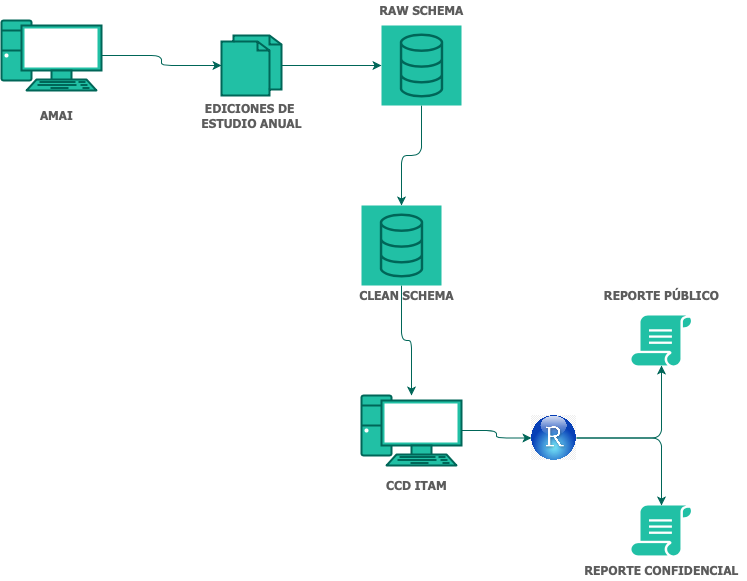
\includegraphics[scale=0.4]{Imagenes/pipeline.png}
\end{center}
\caption{Pipeline del producto de datos materia del proyecto con motivo de la Edición XXII del Estudio de AMAI}
\end{figure}
\

\section{Consideraciones éticas del producto de datos}

Teniendo presente la importancia para la industria de la información recabada en el marco de la Edición XXII (2019-2019) del Estudio Anual de la Industria de Investigación de Mercados y Opinión Pública en México y la sensibilidad de la misma, se realizó el procesamiento y análisis de la información recibida preservando el carácter confidencial de la misma. Para ello, de manera específica se destaca que:

\begin{itemize}
 \item Los datos fueron procesados sin revelar a ninguno de los participantes terceros el contenido de las respuestas del estudio, de manera directa o indirecta.
 \item  La información reunida se empleó para estimaciones o conteos de forma agregada, sin exponer los datos reportados individualmente por las empresas ni sus correspondientes identidades.
 \end{itemize}

\section{Descripción técnica de producto de datos}

La presente sección brinda la descripción a nivel técnico del producto de datos considera el procesamiento de la información, las consideraciones metodológicas y la solución tecnológica establecida para su desarrollo.

\subsection{Consideraciones metodológicas}

A continuación se exponen las consideraciones metodológicas tomadas en cuenta para consolidar los objetivos de negocios descritos en las secciones \ref{obj:bussiness} y \ref{obj:datascience}. Cabe destacar que estos fueron recogidos a su vez y publicados por AMAI en el documento \emph{Estudio AMAI Edicion XXII (2019-2020). Nota Metodológica.}\footnote{Véase \url{http://amai.org/descargas/reporteMetodologicoCliente270520.pdf}}

\subsubsection{Generalidades}

Tal como se ha expresado en la sección \ref{dataproduct:process}, 
por lo que hace a la identificación de los participantes en el Estudio Anual de AMAI a lo largo del tiempo, ésta se realizó con base en una versión homologada del nombre de las empresas. 

\subsubsection{Tamaño del mercado}

En línea con la metodología por AMAI en estudios previos, el dimensionamiento del tamaño del mercado se realizó con base en la facturación (en pesos  mexicanos) de las empresas que conforman el sector de inteligencia de mercado y  opinión para el periodo del estudio. Sobre este punto, la estimación consideró la suma de tres diferentes componentes relativos al tamaño de mercado \emph{calculado}, \emph{estimado} y \emph{supuesto}:

\begin{itemize}
    \item \emph{Calculado:} se refiere a los datos de facturación que fueron proporcionados explícitamente por los informantes en el contexto del estudio,
    \item \emph{Estimado:} relativo a la información de facturación que aunque no fue proporcionada de forma explícita, se tienen datos históricos u otras fuentes que permiten estimarlos en el periodo relevante.
    \item \emph{Supuesto}: corresponde al resto de la industria sobre lo cual se desconocen los datos de facturación.
\end{itemize}

A continuación se describe la metodología adoptada en cada uno de tales
conceptos:\vspace{0.5cm}

\noindent \emph{Metodología para el valor de mercado calculado}

\noindent Se estima como la suma del nivel de facturación reportado por los participantes.\\

\noindent \emph{Metodología para el valor de mercado estimado}

\noindent En primera, se identificaron empresas que 1) contestaron el estudio sin proporcionar datos de facturación, o bien 2) dejaron de participar en dicho  estudio debido a algún motivo y que, por ende, se dejó de tener datos de su facturación en ésta edición.

Posteriormente, se hizo una análisis de la información histórica reunida por AMAI de tales empresas, para identificar los valores de facturación más recientes de los que tuviera noticia para tales empresas, encontrándose que para la mayoría de empresas bajo los supuestos 1) y 2), existen registros de su nivel de facturación en la edición 2018. Sin embargo, para dos empresas los datos encontrados se ubican en periodos más lejanos.

En consideración de ello, para el caso de las empresas donde existe información de su facturación en 2018, el nivel correspondiente al 2019 se estimó aplicando al valor 2018 una tasa ponderada de cambio en el nivel de facturación de ambos periodos, cuyo cálculo se realizó con base en la mediana, en términos porcentuales, de la variación observada sobre la facturación de las empresas para los que si se encontraron datos en 2018 y 2019 (es decir, empresas coincidentes 2018-2019). Esta tasa fue cuantificada en $-3.6\%$.

Se consideró pertinente emplear dicha tasa dada la dinámica observada en el nivel facturación de las empresas coincidentes de 2018 y 2019, la cual se ejemplifica en la figura 3.1, donde se han modificado los nombres de las empresas para respetar los acuerdos de confidencialidad existentes entre AMAI y el CCD del ITAM.

\begin{figure}[h]
\begin{center}
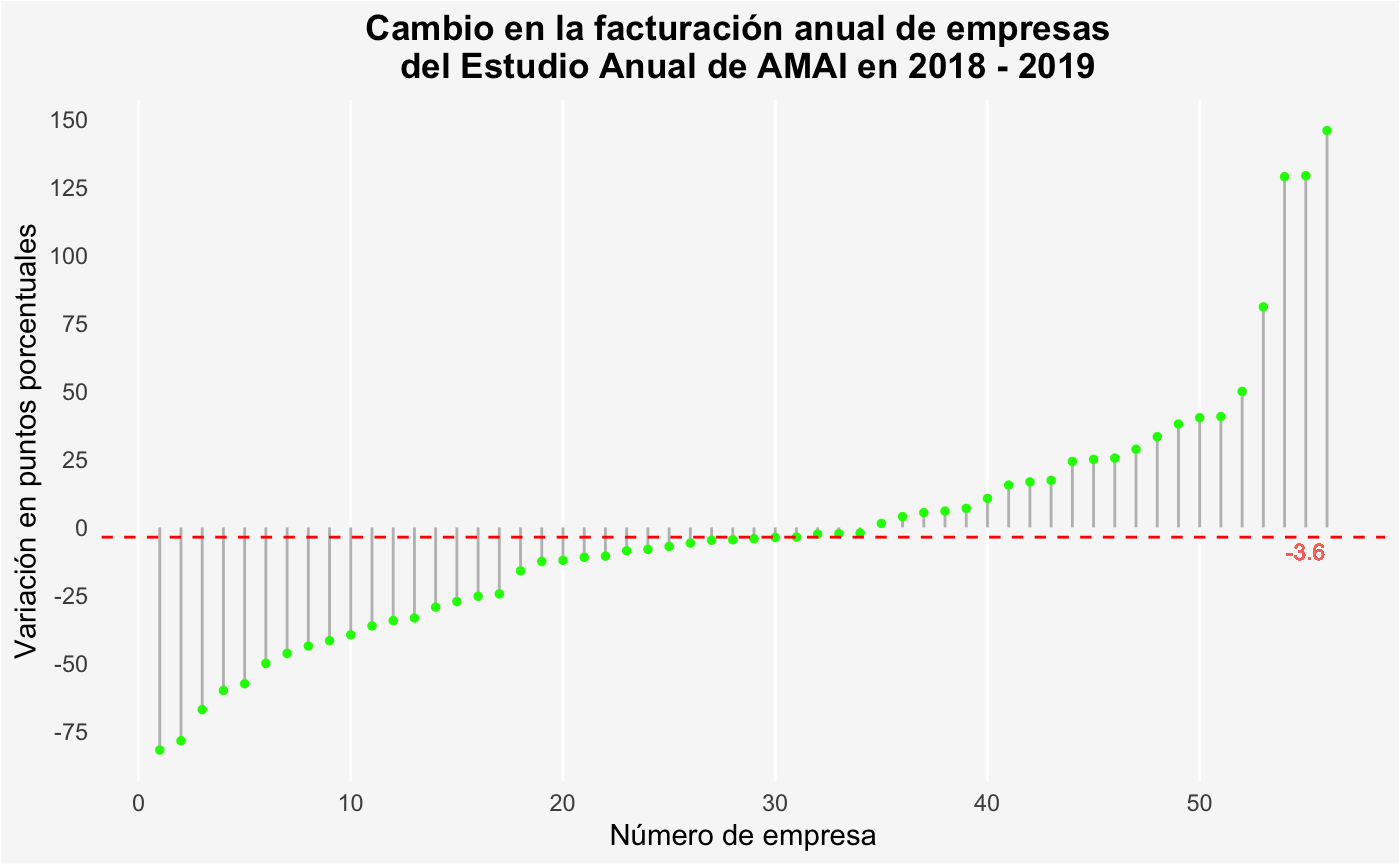
\includegraphics[scale=0.4]{Imagenes/empresas_coincidentes.png}
\end{center}
\caption{Comparación de niveles de facturación de empresas coincidentes 2018-2019 en ambos periodos}
\end{figure}

\newpage

Por otra parte, se hicieron consideraciones particulares sobre dos empresas:

\begin{itemize}
\item En el primer caso se identificó que el último dato de facturación existente se remonta a 2015. Sin embargo, éste valor es menor, en tres órdenes de magnitud, al resto de información histórica de dicha empresa. Ante la evidencia, se consideró que probablemente fue un error de llenado en los datos de facturación para esta empresa, por lo que para 2015 dicho valor se  ajustó multiplicándolo con un factor de 1,000. Adicionalmente, para poder estimar su facturación correspondiente a 2019, sobre el dato de 2015 se aplicaron, de manera consistente con la metodología de AMAI en el estudio 2018, una serie de tasas de crecimiento anual de dicha empresa que fueron reportadas verbalmente a AMAI (9\% a 2016, 8\% a 2017 y 6\% a 2019), así como el valor estimado de crecimiento de facturación de las empresas en el estudio previo (4.7\% a 2018).
\item Para el segundo caso, se identificó que el último valor de facturación reportado corresponde a 2017. En este caso, el valor correspondiente a 2019 se estimó aplicando una tasa ponderada de cambio en el nivel de facturación, empleando la mediana de la variación observada sobre la facturación de las empresas para los que si se encontraron datos en dichos periodos de a) 2017 a 2018 (2\%), y b) 2018 a 2019 (-3.6\%).
\end{itemize}

\noindent \emph{Metodología para el valor de mercado supuesto}

\noindent Se empleó el mismo procedimiento seguido por AMAI en la edición previa del estudio, relativa considerar que la suma  del valor \emph{calculado} y \emph{estimado} equivale al 80\% del mercado total y que, por ende, el mercado \emph{supuesto} se puede obtener como el complemento, es decir, corresponde a 20\% de la facturación de mercado total.

\subsubsection{Mismas empresas reportando}

Dado que sobre este punto, el interés es comparar los cambios en los niveles de facturación para 2018 y 2018, aquí se tomó como referencia a las empresas que reportaron información de facturación en el periodo 2019 del estudio y en el previo.

A continuación se describe la metodología seguida para realizar comparativos de interés al respecto.\\

\noindent \emph{Diferencias vs año anterior}

Estimado como la diferencia numérica en los datos de facturación de 2018 y 2019, para las empresas coincidentes en ambos periodos.\\

\noindent \emph{Desempeño vs año anterior}

Calculado como la diferencia porcentual entre los datos de facturación de 2018 y 2019, para las empresas coincidentes en ambos periodos.

\subsubsection{Valor de tamaño de mercado}

\begin{itemize}
\item Para los datos de periodos hasta 2018, se empleó la información histórica generada por AMAI en las ediciones pasadas del estudio.

\item Para 2019, se tomó como referencia al proceso descrito en el apartado \textbf{Tamaño del mercado} de la presente sección para el dimensionamiento del tamaño del mercado.
\end{itemize}

\noindent \emph{Tendencia de valor nominal y real de la industria}

En línea con la metodología desarrollada en la edición pasada del estudio, para estimar el valor del tamaño del mercado en términos reales, se realizaron los siguientes pasos:

\begin{itemize}
    \item El valor nominal se consideró de acuerdo al valor estimado de dicha cantidad para 2019, conforme a la exposición realizada en el apartado \textbf{Tamaño del mercado} de la presente sección,
    \item El índice nacional de precios al consumidor publicado por el Instituto Nacional de Estadística y Geografía (INEGI), con base en la segunda quincena de julio de 2018\footnote{Disponible a través de la dirección electrónica \url{https://www.inegi.org.mx/sistemas/bie/}, mediante
la ruta \textit{Indicadores económicos de coyuntura, Índices de precios , Índice nacional de precios al consumidor. Base segunda quincena de julio de 2018=100, Mensual, Índice, Índice general}}.
\end{itemize}

\noindent \emph{Variaciones porcentuales anuales en el valor de la industria}

El cálculo de este punto se estimó como la diferencia porcentual entre los datos de valor de mercado, en términos nominales, de 2013 a 2019, con diferencia de un año. En tal sentido, para el valor nominal del mercado se consideró lo siguiente:

\begin{itemize}
\item  Hasta 2018, se emplearon los datos del valor del mercado estimado en los estudios de AMAI, 
\item  Para 2019, se usó la estimación del CCD del ITAM, conforme al proceso descrito en el apartado \textbf{Tamaño del mercado} de la presente sección.
\end{itemize}

\noindent \emph{Variaciones porcentuales anuales (mismas empresas reportando)}

Análogamente, este punto fue estimado como la diferencia porcentual entre los datos de facturación agregada las empresas coincidentes periodos con diferencia de un año, considerando datos que abarcan de 2013 a 2019. Por lo que hace a los datos del valor nominal del mercado se consideró lo siguiente:

\begin{itemize}
\item Para valores el valor nominal hasta 2018, se emplearon los datos del valor del mercado estimado en los estudios de AMAI, 
\item Para 2019, se usó la estimación del CCD del ITAM, conforme al proceso descrito en el apartado \textbf{Tamaño del mercado} de la presente sección.
\end{itemize}

\noindent \emph{Tendencia de valor nominal de la industria (en dólares americanos)}
Valor nominal del mercado:
\begin{itemize}
\item Para valores hasta 2018, se emplearon los datos del valor del mercado estimado en los estudios de AMAI, 
\item Para 2019, se usó la estimación del valor del mercado total, calculada por el CCD del ITAM para 2019 con la metodología descrita en el apartado \textbf{Tamaño del mercado} de la presente sección.
\end{itemize}

\noindent Tipo de cambio dolar americano a pesos mexicanos:

\begin{itemize}
\item Hasta el año 2018, se emplearon datos reportados de tipo de cambio reportados por el Banco Mundial\footnote{Véase \url{https://datos.bancomundial.org/indicador/PA.NUS.FCRF?locations=MX}}

\item En complemento, para la estimación del 2019, se usó como base al \emph{Tipo de cambio (Fix) para solventar obligaciones denominadas en dólares de los EE.UU.A., pagaderas en la República Mexicana} publicado por el Banco de México\footnote{Véase \url{https://www.banxico.org.mx/tipcamb/main.do?page=tip&idioma=sp} }, calculado considerando promedio de los valores promedio reportados en los días de cada mes, al 24/04/2020.

\end{itemize}

\subsubsection{Volumen de mercado}

\noindent \emph{Volumen de producción}

Para este punto, se contabilizó el total cantidad de unidades reportadas por los participantes del estudio, considerando el total del proyectos realizados en la industria, así como el número de 1) sesiones de grupo presenciales o remotas, 2) entrevistas a profundidad y 3) etnografías o aplicaciones de antropología.

En torno a las sesiones de grupo presenciales o remotas, de la revisión a las respuestas se identificó que un participante reportó haber llevado a cabo cerca de 479,000 sesiones. Al contrastarlo, se encontró que i) considerando las sesiones de grupo reportadas por las empresas en su conjunto, dicha cantidad equivaldría al 98\% de las mismas, mientras que ii) 75\% de las empresas en el estudio tiene a lo más 200 sesiones de grupo.

Es así que ante la posibilidad de que el valor aludido fuera un error de captura se excluyó la respuesta del participante en comento para consolidar el conteo de sesiones de grupo presenciales o remotas.\\

\noindent \emph{Tipo de entrevistas}

Con referencia a este rubro, se contabilizaron los diferentes tipo de entrevistas realizadas (a saber, por Internet, cara a cara en domicilios, vía pública, telefónico y salida de casilla), para posteriormente estimar la correspondiente distribución porcentual de los mismos. 

\subsubsection{Capital humano}

Para la estimación de este concepto, se contabilizó la cantidad de recursos humanos reportados por los participantes del estudio en los diversos segmentos que integran una empresa, esto es, socios y altos ejecutivos, personal técnico y de atención a clientes, de apoyo administrativo y equipo de producción, considerando el desglose por género dentro de cada uno de tales segmentos.\\

\noindent \emph{Distribución de capital humano}

A partir de dicha información, se calcula el número total de recursos humanos en la industria junto con su distribución por segmento.

\subsubsection{Ranking de empresas}

Estimado considerando a las empresas que reportaron explícitamente su nivel de facturación en 2019 y que además otorgaron su consentimiento expreso para formar parte del ranking. 

En este sentido, el ranking se formó considerando las posiciones de las empresas ordenadas de mayor a menor según el nivel de facturación reportado para el periodo del estudio, pero sin revelar el dato concreto de facturación de cada empresa para preservar la confidencialidad de dicha información.

\subsubsection{Ante la incertidumbre futura}

\begin{itemize}
\item Con respecto a este punto, se realizó un análisis de texto que permitió identificar los temas que fueron mayormente abordados en las respuestas de los participantes del estudio 2019, como retos, cambios y temas de innovación para la industria.
\item Como resultado, se reportaron 1) los 10 términos más frecuentes, 2) un resumen ejecutivo de los comentarios vertidos por los participantes en torno a los términos más frecuentes, y 3) una nube de palabras para facilitar la exposición del vocabulario empleado por los mismos, donde el tamaño y color de los términos fue proporcional a su frecuencia\footnote{Para este punto, se eliminaron \emph{stopwords} y caracteres de puntuación, considerándose en el ejercicio unigramas y bigramas, empleando las librerias SnowballC, Wordcloud y RColorBrewer de R}.
\end{itemize}

\subsubsection{Perspectivas 2020}

\begin{itemize}
\item Sobre este tema, el estudio 2019 reúne las perspectivas de los informantes a través de diferentes temas: I) Mi empresa, II) México en general, III) Industria en el mundo, IV) Industria en México y  V) Economía personal,
\item Tales perspectivas son consideradas a través de las etiquetas \emph{igual}, \emph{mejor} y \emph{peor} que limitan las respuestas de las empresas,
\item Considerando tales puntos, se realizaron conteos de las mismas para establecer cantidades totales y proporciones de las perspectivas de dichos temas a través del conteo de las respuestas empleando tales etiquetas.
\end{itemize}

\subsection{Consideraciones tecnológicas}

Para el desarrolló de este proyecto hizo uso de infraestructura de servicios de computación en la nube a través del proveedor Amazon Web Services (AWS), contratados por el CCD del ITAM. En concreto se echaron mano de los siguientes:

\begin{enumerate}
    \item \emph{Amazon S3, Amazon Simple Storage Service o Bucket} es un servicio que proporciona una interfaz de almacenamiento de archivos, en donde se depositaron los datos correspondientes a las diferentes ediciones del Estudio Anual de AMAI. 
    \item \emph{Amazon Elastic Compute Cloud  o EC2} el cual consiste en poner a disposición de los usuarios una máquina virtual con diferentes configuraciones de hardware, espacio y sistema operativo. En este caso se empleó una instancia de uso general, con 8 GB de ram, 4 cores y Ubuntu 18.04.4 LTS.
    \item \emph{Amazon Relational Database Service} se trata de un servicio de base de datos relacional; particularmente se empleó un servicio con una base PostgreSQL, a través del cliente \emph{psql} desde conexión SSH hacia la instancia EC2. 
    \item Todos estos servicios se encontraron inmersos dentro de una \emph{Amazon Virtual Private Cloud (VPC)} que proporciona un entorno restringido de trabajo, para garantizar la seguridad de la información y desarrollos realizados.
\end{enumerate}

Para facilitar el entendimiento a continuación se presenta un diagrama\footnote{Elaborado a través de Arcentry, \url{https://arcentry.com/?src=aws}} de los servicios empleados y de su interrelación:

\begin{figure}[h]
\begin{center}
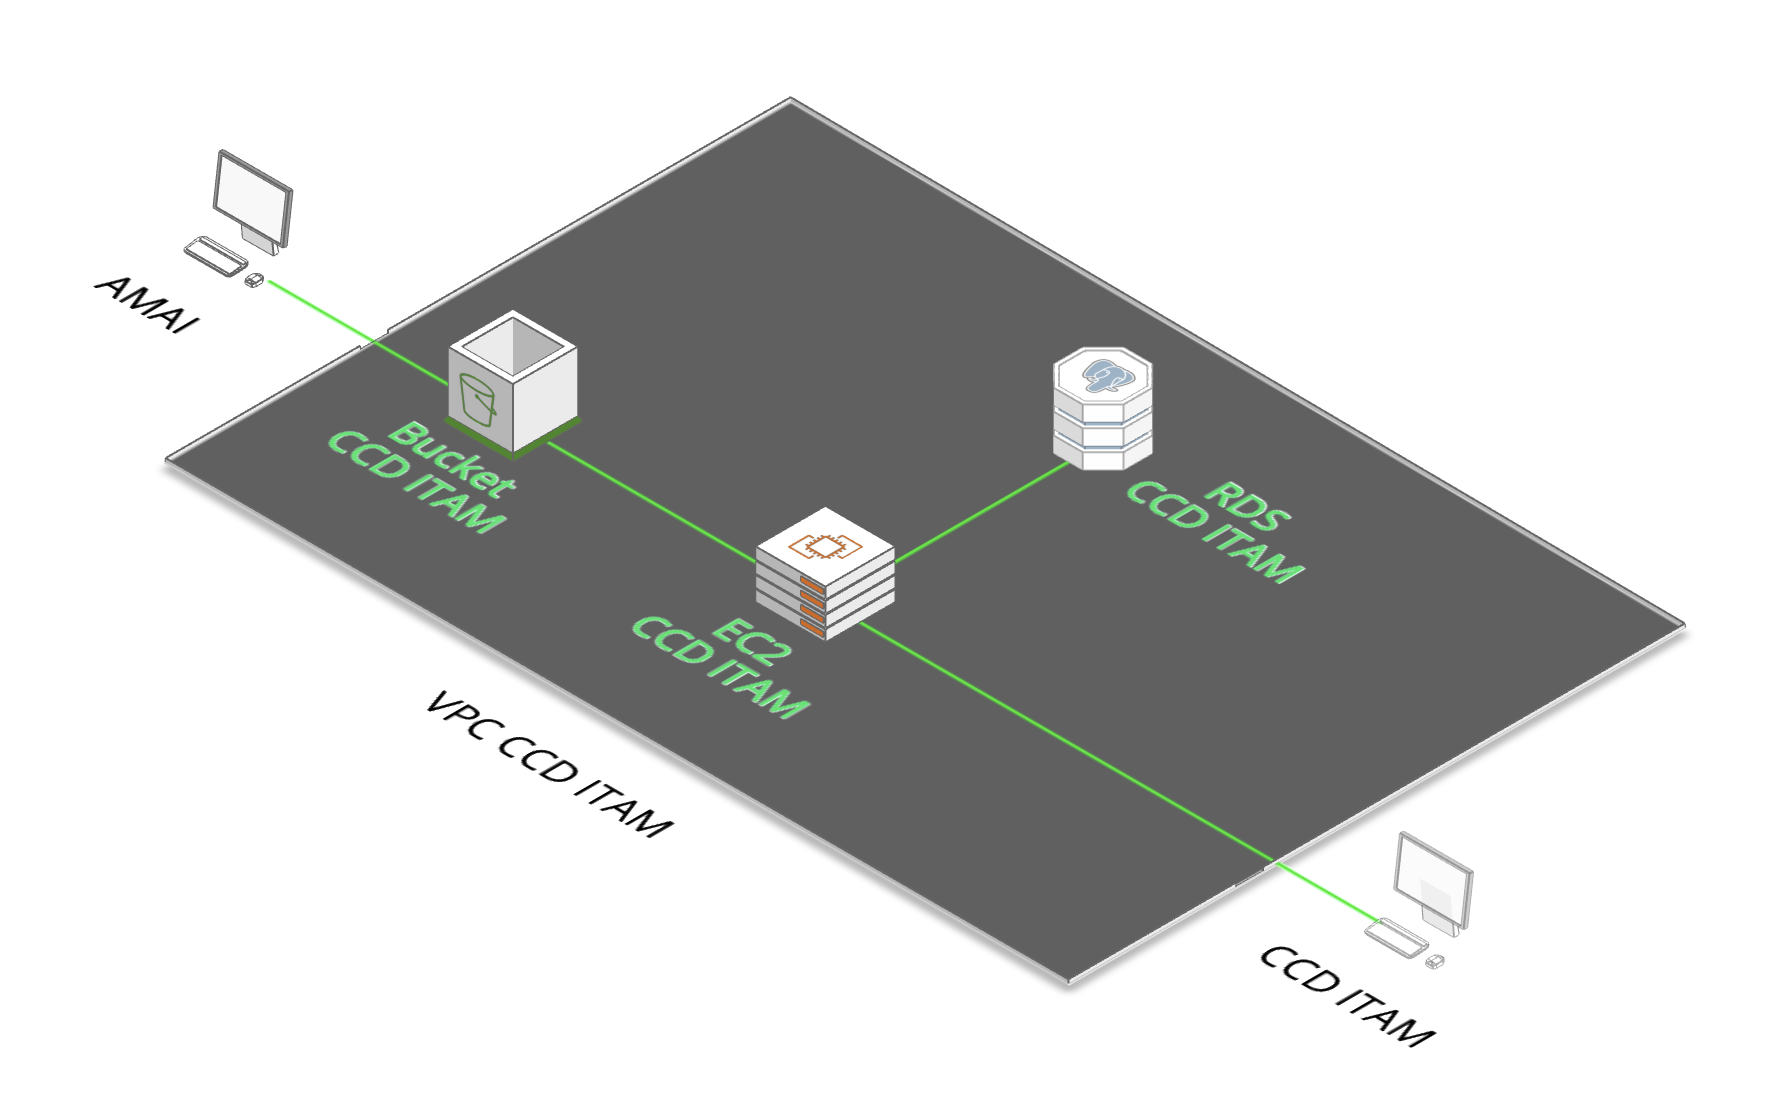
\includegraphics[scale=0.4]{diagrama_aws.png}
\end{center}
\caption{Diagrama de servicios de AWS utilizados por el CCD del ITAM para el proyecto}
\end{figure}

\chapter{Resultados}

\noindent En este último capítulo presenta los resultados obtenidos en el desarrollo del proyecto. Cabe destacar que debido al acuerdo de confidencialidad existente entre AMAI y el CCD del ITAM sólo se comunicarán resultados que fueron publicados en referencia al Estudio XXII (2019-2020) del Estudio Anual de AMAI, a través del documento \emph{Estudio Anual de la Industria de Investigación de Mercados y Opinión Pública en México. Edición XXII (2019-2020).}\footnote{\url{https://www.amai.org/descargas/Estudio_Anual_AMAI_XXII_Edicion_2019_Comunicado_Medios_Junio_2020.pdf}}. El resto de resultados se ha compartido a manera de un reporte ejecutivo para las empresas participantes en el consabido estudio.

\section{Valor del mercado}

\begin{itemize}
    \item En 2019 la industria de investigación de mercados e inteligencia aplicada al consumidor en México alcanzó un valor anual de 7,664 millones de pesos.
    \item En esta edición hubo 71 empresas que participaron.
    \item Es posible hacer comparaciones directas de 61 empresas que participaron en la Edición XXII (2018-2019) y la Edición XXII (2019-2020) del Estudio Anual de AMAI.
    \item Las empresas comparables entre ambos periodos tuvieron un crecimiento orgánico de 0.81\%.
    \item Hablando de dichas empresas comparables, 56\% reportaron decrecimiento mientras que 44\% observaron un crecimiento.
\end{itemize}

\section{Distribución y volumen mercado}

\begin{itemize}
\item De acuerdo a los datos Edición XXII (2019-2020) del Estudio Anual de AMAI, en México sigue predominando la investigación de mercado basada en investigación de corte cuantitativo, que representa alrededor de 67\% de la facturación anual.
\item En 2019 se hicieron 9 mil proyectos de investigación e inteligencia de mercados, casi el mismo número que la edición anterior indicando que si bien no hubo un aumento tampoco hubo disminución en proyectos. 
\item Por lo que hace a unidades de investigación cualitativa se realizaron 9 mil sesiones de grupo, 13 mil entrevistas a profundidad y 4 mil observaciones etnográficas.
\item El número de entrevistas con informantes de proyectos de investigación en 2019 es de 7 millones de contactos efectivos. Las entrevistas personales -cara a cara más vía pública- continúan siendo las predominantes con 3.17 millones de contactos que representan aproximadamente el 43\% de la forma de contacto. En segundo lugar, se encuentran los puntos de contacto por Internet con 2.75 millones de contactos.
\end{itemize}


\section{Capital Humano}

\begin{itemize}
\item El capital humano para la Edición XXII (2019-2020) del Estudio Anual de AMAI estuvo conformado por casi 11 mil personas, que corresponde a una disminución de aproximadamente 61\% con respecto a la edición pasada\footnote{Aparentemente se debe al contexto de elecciones en el ejercicio previo, donde la mayor parte del personal activo se contrató de manera eventual}, e inclusive un poco más bajo que en entregas anteriores a la Edición XXI (2018-2019) donde había entre 12 y 15 mil personas en la industria.
\item Con respecto a la distribución del capital humano en términos de su género, es grato compartir que por primera vez, la proporción de hombres y mujeres es 1, es decir, por cada hombre hay una mujer. 

\item En esta edición los tipos de personal que en la edición anterior tuvieron más hombres que mujeres correspondientes a segmentos operativos y de producción, tuvieron una proporción de 1 y 1 respectivamente.
\end{itemize}

\section{Ranking de empresas}

A continuación se listan en esta tabla solamente aquellas empresas que expresamente manifestaron su aceptación de estar en este listado. En este sentido, este ranking no tiene el valor representativo de otros indicadores del Estudio Anual. 

Dicho listado se ha construido a partir de un orden, de mayor a menor, de facturación reportada; con lo cual la disposición de las empresas en orden no implica necesariamente una posición de mayor o menor calidad, prestigio o cualquier otro criterio que no sea el de la facturación reportada.

\begin{table}[]
\caption{Ranking de empresas participantes en Edición XXII (2019-2020) del Estudio Anual de AMAI (parte 1)}
\label{tab:ranking1}
\begin{tabular}{|l|l|}
\hline
Empresa                                                            & Rank \\ \hline
IPSOS                                                              & 1    \\ \hline
UPAX SA DE CV                                                      & 2    \\ \hline
DE LA RIVA                                                         & 3    \\ \hline
ESTADISTICA APLICADA                                               & 4    \\ \hline
SMART INDEX                                                        & 5    \\ \hline
O’ DE LA ROQUETTE                                                  & 6    \\ \hline
LEXIA INSIGHTS \& SOLUTIONS                                        & 7    \\ \hline
MARKETING GROUP                                                    & 8    \\ \hline
G DE VILLA Y ASOCIADOS SAPI DE CV                                  & 9    \\ \hline
GFK MEXICO                                                         & 10   \\ \hline
BRAIN                                                              & 11   \\ \hline
AAGA MARKETING                                                     & 12   \\ \hline
PEARSON                                                            & 13   \\ \hline
NETQUEST                                                           & 14   \\ \hline
PHENOMA                                                            & 15   \\ \hline
SERTA MARKETING INTELLIGENCE PATTNER                               & 16   \\ \hline
EL INSTITUTO DE INVESTIGACIONES SOCIALES SC                        & 17   \\ \hline
\parbox[t]{11cm}{NODO INVESTIGACION ESTRATEGICA SUASOR CONSULTORES}                  & 18   \\ \hline
SUASOR CONSULTORES                                                 & 19   \\ \hline
\parbox[t]{11cm}{ESTUDIOS DE VARIABLES DEL MERCADO SC BERUMEN Y ASOCIADOS S A DE CV} & 20   \\ \hline
\end{tabular}
\end{table}


\begin{table}[]
\caption{Ranking de empresas participantes en Edición XXII (2019-2020) del Estudio Anual de AMAI (parte 2)}
\label{tab:ranking2}
\begin{tabular}{|l|l|}
\hline
Empresa                                                      & Rank \\ \hline
BERUMEN Y ASOCIADOS S A DE CV                                & 21   \\ \hline
PQR PLANNING QUANT                                           & 22   \\ \hline
FOCUS INVESTIGACION DE MERCADOS                              & 23   \\ \hline
INTEGRACION TOTAL                                            & 24   \\ \hline
MARES CONSUMER INTELLIGENCE                                  & 25   \\ \hline
INMEGA DESARROLLO DE NEGOCIOS                                & 26   \\ \hline
MERCAEI                                                      & 27   \\ \hline
QUESTIONPRO LATINOAMERICA                                    & 28   \\ \hline
\parbox[t]{11cm}{CUARTEL GENERAL DE INVESTIGACION DE MERCADOS MASTER RESEARCH} & 29   \\ \hline
MASTER RESEARCH                                              & 30   \\ \hline
PSYMA LATINA                                                 & 31   \\ \hline
FACTA RESEARCH                                               & 32   \\ \hline
EVIDENS CONSULTORIA DE MARCA                                 & 33   \\ \hline
GAIN DYNAMICS RESEARCH                                       & 34   \\ \hline
ENKOLL                                                       & 35   \\ \hline
DINAMIA                                                      & 36   \\ \hline
CINCO                                                        & 37   \\ \hline
INMERSA MARKETING GROUP                                      & 38   \\ \hline
ACSI RESEARCH                                                & 39   \\ \hline
IMAAC MARKETING GROUP                                        & 40   \\ \hline
\end{tabular}
\end{table}

\begin{center}
\begin{table}[h]
\caption{Ranking de empresas participantes en Edición XXII (2019-2020) del Estudio Anual de AMAI (parte 3)}
\label{tab:ranking3}
\begin{tabular}{|l|l|}
\hline
Empresa                   & Rank \\ \hline
SINCRONIA                 & 41   \\ \hline
ISOPOMER                  & 42   \\ \hline
MEBA                      & 43   \\ \hline
WISUM                     & 44   \\ \hline
GAUSSC                    & 45   \\ \hline
NEUROMARKETING            & 46   \\ \hline
SEGMENTOS RESEARCH        & 47   \\ \hline
SURVEY                    & 48   \\ \hline
OVALBOX                   & 49   \\ \hline
SEMIOSFERA CONSULTING S C \hspace{4cm} & 50   \\ \hline
\end{tabular}
\end{table}
\end{center}

\newpage
% Gráfica con dos colores a mano

\section{Documentos generados para AMAI}

Por otra parte, cabe destacar que como resultado del proyecto recién descrito, se entregaron dicha asociación una serie de documentos que contienen los resultados generados con el producto de datos diseñado para la Edicion XXII del Estudio Anual de AMAI:

\begin{enumerate}
    \item \emph{Estudio Anual de la Industria de Investigación de Mercados y Opinión Pública en México. Edición XXII (2019-2020). Nota metodológica.}\footnote{Disponible a través de la dirección electrónica: \url{http://amai.org/descargas/reporteMetodologicoCliente270520.pdf}}
    \item \emph{Estudio Anual de la Industria de Investigación de Mercados y Opinión Pública en México. Edición (2019-2020). Comunicado a Medios.}\footnote{Véase \url{https://www.amai.org/descargas/Estudio_Anual_AMAI_XXII_Edicion_2019_Comunicado_Medios_Junio_2020.pdf}}
    \item \emph{Estudio Anual de la Industria de Investigación de Mercados y Opinión Pública en México. Edición (2019-2020). Reporte a Participantes}
\end{enumerate}

Sobre éste último documento, cabe destacar que debido al acuerdo de confidencialidad existente entre AMAI y el CCD los resultados se reservaron para participantes en el estudio debido al carácter confidencial de la información, sin embargo su contenido versa sobre los elementos de valor obtenidos en el estudio con referencia a los puntos descritos en la sección \ref{obj:bussiness}.

\chapter*{Conclusiones y Recomendaciones}
\addcontentsline{toc}{chapter}{Conclusiones y Recomendaciones}

A continuación se presentan las conclusiones y recomendaciones asociadas al proyecto materia del presente trabajo.

% Las conclusiones tampoco cuentan como capítulo

\section*{Conclusiones}

\begin{itemize}
    \item En este documento se ha presentado un producto de datos encaminado a calcular y determinar diferentes elementos de valor para la industria  de investigación de mercados e inteligencia aplicada al consumidor en México, a partir de las ediciones históricas del Estudio Anual de la Industria de Investigación de Mercados y Opinión Pública en México.
    \item El producto de datos se ha empleado para consolidar reportes ejecutivos de la Edición XXII (2019-2019), dirigidos tanto para el público interesado\footnote{Véase \url{ttps://www.amai.org/descargas/Estudio_Anual_AMAI_XXII_Edicion_2019_Comunicado_Medios_Junio_2020.pdf}} y otro confidencial, restringido hacia los participantes del estudio, pues contiene información de coyuntura para la industria.
    \item A partir de dicha información se desarrolló código en SQL y R, a través del cual se determinaron diferentes elementos clave a partir de la Edición XXII del estudio en cuestión, entre los cuales destacan 1) el dimensionamiento del volumen del mercado en 2019, según la facturación alcanzada en dicho periodo, 2) la cantidad de proyectos cualitativos y cuantitativos, según su tipo, 3) la cantidad de unidades realizadas para estudios cualitativos, así como en el caso de estudios cuantitativos, la cantidad de entrevistas realizado de acuerdo al tipo correspondiente, 4) la composición de los recursos humanos la industria, en todos sus segmentos, considerando la desagregación por género, 5) identificación de principales retos, cambios y temas prioritarios a futuro para la industria en el mediano plazo, 6) el ranking de empresas de acuerdo a su nivel de facturación en 2019. 
    
    \item Cabe destacar que en este punto anterior, se involucraron estimaciones de inferencia, a manera de, cálculos agregados, así como análisis de texto.
    
    \item Finalmente, se encontraron diversos cambios en la situación de este mercado, entre los que destacan: 1) un ligero crecimiento en el valor del mercado, aunque para las empresas que participaron en la Edicióon  XXII  (2018-2019)  y  la  Edicóon  XXII(2019-2020) del Estudio Anual de AMAI (0.81\%), la mayoría de ellas decrecieron, 2) en México sigue predominando la investigación de  mercado  basada  en  corte  cuantitativo (que representa 67\% de facturación anual), 3) hablando del capital humano de la industria, se observó un disminución del 61\% de los recursos humanos, sin embargo por primera ves la proporción de hombres y mujeres es 1 a 1. 
    
\end{itemize}


\section*{Recomendaciones}

\begin{itemize}

    \item Para desarrollar el estudio con conocimiento preciso del significado de las variables involucradas, es necesario consolidar documentación de las bases de datos que reúnen las respuestas de los participantes. Para avanzar en dicha dirección, se puede retomar el material presentado en la sección \ref{data:sources}.

    \item Es deseable añadir identificadores de las empresas a las bases de datos que recogen la respuesta del estudio, para encontrarse en condiciones de unir con facilidad datos de diferentes ediciones del estudio.
    
    \item Las preguntas del Estudio Anual de AMAI pueden ampliarse para considerar la circunstancias actuales pues determinan nuevos temas de conyuntura como el impacto de Covid 19, la digitalización de servicios y el uso de nuevas tecnologías.
    
\end{itemize}



%----------------------------------------------------------------------------------------
%	APÉNDICES
%----------------------------------------------------------------------------------------

\begin{appendix}

\chapter{Censo de la Industria de la Investigación de Mercados y Opinión Pública 2019} \label{censo2019}

\textbf{Nota:} El texto siguiente corresponde a la Edición XII (2019-2019) del Estudio Anual de la Industria de Investigación de Mercados y Opinión Pública en México\footnote{Fuente: Asociación Mexicana de Agencias de Inteligencia de Mercado y Opinión A.C. (“AMAI”), a través del Centro de Ciencia de Datos ITAM}.\newline


\noindent Este CENSO ha sido promovido por la AMAI con la finalidad de contar con una estimación lo más certera posible del volumen y características de la industria de investigación de mercados y opinión pública en México.
A partir de los datos de este censo, la AMAI elaborará un documento del estado de nuestro mercado, mismo que será difundido a los participantes del ejercicio, los medios de comunicación y los interesados en México y el extranjero.

Dada la naturaleza de la información que se pide, este cuestionario está dirigido al Presidente, Director General o socio principal de la empresa. Los datos recabados serán mantenidos en confidencialidad.
Sólo se divulgarán públicamente datos agregados y no información específica de una empresa en particular.

En el caso de la facturación, según la política adoptada desde el año 2002, para la difusión pública se hará un rankeo, sin especificar cifras, de aquellas empresas que expresamente lo autoricen.\newline

I. CONFIDENCIALIDAD DE LOS DATOS\newline

1.- ¿Autoriza que el nombre de su empresa aparezca en el rankeo público de compañías de investigación, ubicando su lugar a partir del dato de facturación proporcionado, pero sin revelarlo públicamente? (obligatoria)

SELECCIONE SOLAMENTE UNA OPCIÓN
\begin{itemize}
    \item[1)] (\rule{20mm}{0.1mm}) Sí
    \item[2)] (\rule{20mm}{0.1mm}) No
\end{itemize}

2.- Nombre oficial de la empresa (obligatoria)\newline

3.- Nombre del informante (obligatoria)\newline

II. TIPOS DE INVESTIGACIÓN REALIZADA\newline
4.- ¿En 2019 su empresa realizó proyectos bajo los siguientes tipos de investigación? (obligatoria)

\begin{itemize}
    \item[A)] Cualitativos a partir de interacciones con informantes: incluye sesiones de grupo, entrevistas a profundidad, etnografía aplicada, ya sea presencial o remota (por ejemplo: en línea), observaciones de conductas de consumo o procesos de venta (compras simuladas), etcétera
    \item[B)] Cuantitativos a partir de entrevistas con informantes: incluye todo tipo de proyectos hechos a partir de entrevistas estructuradas con grupos amplios de informantes, seleccionados aleatoriamente o bajo otro tipo de procedimiento. Las entrevistas pudieron haberse hecho cara a cara o en forma remota (telefónicamente, en línea, etcétera)
    \item[C)] Recolección y analítica de datos, tanto primarios como secundarios. Incluye auditorías de ventas y análisis de compraventas realizadas por bases de datos de clientes de una compañía; análisis de big data y otros relacionados, modelación de conductas y procesos de compra para productos de un cliente, etcétera
    \item[D)] Aplicaciones de biometría o neurociencia para determinar respuestas a estímulos diversos o para apoyar la realización de proyectos encaminados a entender o generar una determinada decisión humana
    \item[E)] Servicios de consultoría, asesoría o capacitación que se hayan facturado independientemente de proyectos de investigación de mercados y opinión pública
\end{itemize}

III. FACTURACIÓN EN 2019\newline

DESCONTAR FACTURACIÓN CRUZADA ENTRE FILIALES Y SUBCONTRATACIÓN A OTRAS EMPRESAS DE INVESTIGACION QUE NO SON MAQUILADORES. EN CASO DE CORPORATIVOS, CONSOLIDAR LA FACTURACION DE TODAS LAS UNIDADES DE NEGOCIO

5.- Por favor escriba con número el TOTAL de la facturación que tuvo su empresa en 2019. NOTA: Utilizar solamente dígitos, sin comas, espacios, ni signos de pesos. (obligatoria)
1) \rule{20mm}{0.1mm} pesos mexicanos

6.- Por favor escriba el porcentaje aproximado de la facturación total que tuvo su empresa en 2019. NOTA: El total de los porcentajes deberá sumar 100\%. (obligatoria)
VERIFIQUE QUE LA SUMA SEA 100\%

\begin{itemize}
    \item[1)] \rule{20mm}{0.1mm} \% Del total en Proyectos CUALITATIVOS
\item[2)] \rule{20mm}{0.1mm} \% Del total en Proyectos CUANTITATIVOS
\item[3)] \rule{20mm}{0.1mm} \% Del total en RECOLECCIÓN Y ANALÍTICA DE DATOS
\item[4)] \rule{20mm}{0.1mm} \% Del total en APLICACIONES DE BIOMETRÍA O NEUROCIENCIA
\item[5)] \rule{20mm}{0.1mm} \% Del total en servicios de CONSULTORÍA, asesoría o capacitación
\item[6)] \rule{20mm}{0.1mm} \% Otros
\end{itemize}

\rule{20mm}{0.1mm} \% TOTAL

7- De acuerdo a su mejor estimación, por favor indique qué porcentaje de su facturación anual total en 2019 correspondió a los siguientes rubros:\newline

1) DESTINATARIO

\rule{20mm}{0.1mm} \% del total

\begin{itemize}
    \item[a)] Para clientes o peticionarios establecidos en México \rule{20mm}{0.1mm}
\item[b)] Para clientes o peticionarios de países extranjeros \rule{20mm}{0.1mm}
\end{itemize}

2) SECTOR

\begin{itemize}
    \item[a)] Sector público / gobierno de México u otro país
\item[b)] Sector privado de México u otro país \rule{20mm}{0.1mm}
\item[c)] ONGs o instituciones similares de México u otro país \rule{20mm}{0.1mm}
\end{itemize} 

3) INDUSTRIA

\begin{itemize}
    \item[a)] Productos de consumo perecederos \rule{20mm}{0.1mm}
\item[b)] Productos de consumo no perecederos \rule{20mm}{0.1mm}
\item[c)] Comercio y menudeo \rule{20mm}{0.1mm}
\item[d)] Servicios financieros \rule{20mm}{0.1mm}
\item[e)] Automotriz \rule{20mm}{0.1mm}
\item[f)] Farmaceútica \rule{20mm}{0.1mm}
\item[g)] Telecomunicaciones y tecnología de comunicación \rule{20mm}{0.1mm}
\item[h)] Medios de comunicación y entretenimiento \rule{20mm}{0.1mm}
\item[i)] Agencias de publicidad \rule{20mm}{0.1mm}
\item[j)] Otros \rule{20mm}{0.1mm}
\end{itemize} 
IV. VOLUMEN DE INVESTIGACIÓN \newline

INVESTIGACIÓN CUALITATIVA HECHA EN 2019 \newline

8. Por favor indique su mejor estimación sobre el volumen de investigación cualitativa hecha por su empresa en 2019: \rule{20mm}{0.1mm} (NO INCLUIR EN ESTE RECUENTO PROYECTOS HECHOS PARA OTRA EMPRESA DE INVESTIGACION DE MEXICO, PERO INCLUIR LAS QUE SE HICIERON COMO MAQUILA PARA CLIENTES EXTRANJEROS).\newline

TIPO DE METODOLOGÍA \newline
UNIDADES REALIZADAS EN 2019 

\begin{itemize}
    \item Sesiones de grupo presenciales o remotas: \rule{20mm}{0.1mm}
\item Entrevistas a profundidad: \rule{20mm}{0.1mm}
\item Etnografías o aplicaciones de antropología: \rule{20mm}{0.1mm}
\end{itemize} 

9. Número de proyectos de investigación cualitativa realizados en 2019: \rule{20mm}{0.1mm} \newline 

INVESTIGACIÓN CUANTITATIVA HECHA EN 2019 \newline

10- Por favor indique su mejor estimación sobre el volumen de investigación cuantitativa hecha por su empresa en 2019: \rule{20mm}{0.1mm} (NO INCLUIR EN ESTE RECUENTO PROYECTOS HECHOS PARA OTRA EMPRESA DE INVESTIGACION DE MEXICO, PERO INCLUIR LAS QUE SE HICIERON COMO MAQUILA PARA CLIENTES EXTRANJEROS)\newline

TIPO DE LEVANTAMIENTO\newline
NÚMERO DE UNIDADES REALIZADAS \newline

\begin{itemize}
    \item Cara a cara en domicilios (viviendas o empresas) \rule{20mm}{0.1mm}
    \item Telefónico \rule{20mm}{0.1mm}
    \item En vía pública / punto de afluencia \rule{20mm}{0.1mm}
    \item A la salida de casilla electoral \rule{20mm}{0.1mm}
    \item Por internet (con personas o empresas) \rule{20mm}{0.1mm}
    \item Otro \rule{20mm}{0.1mm}
\end{itemize}

11.- Número de proyectos cuantitativos que su empresa realizó en 2019, (obligatoria)
      1) \rule{20mm}{0.1mm}  Proyectos cuantitativos con entrevistas\newline
      
V. RECURSOS HUMANOS Y TÉCNICOS \newline

12A.- ¿Cuántas personas colaboraron en su empresa en 2019 de forma permanente, POR NOMINA dentro de los siguientes rubros? (obligatoria) \rule{20mm}{0.1mm} \newline

12B.- De ese personal de planta, que se le paga POR NOMINA, ¿qué porcentajes corresponden a mujeres y a hombres? (haga su mejor estimación)\newline

CATEGORÍA

\begin{itemize}
    \item[1)] Socios y altos ejecutivos (directores generales y directores de área) NÚMERO TOTAL \rule{20mm}{0.1mm} \% MUJERES, \rule{20mm}{0.1mm} \% HOMBRES
    \item [2)] Personal técnico y de atención a clientes (subdirectores, investigadores, analistas, etc.) NÚMERO TOTAL \rule{20mm}{0.1mm} \% MUJERES, \rule{20mm}{0.1mm} \% HOMBRES
    \item [3)] Personal de apoyo administrativo (contadores, secretarias, mensajeros, choferes, etc.) NÚMERO TOTAL \rule{20mm}{0.1mm} \% MUJERES, \rule{20mm}{0.1mm} \% HOMBRES
    \item [4)] Equipo de producción (entrevistadores, capturistas, codificadores) NÚMERO TOTAL \rule{20mm}{0.1mm} \% MUJERES, \rule{20mm}{0.1mm} \% HOMBRES
\end{itemize}
 
GRAN TOTAL \rule{20mm}{0.1mm}


13A.- ¿Cuántas personas colaboraron en su empresa en 2019 eventualmente, POR PROYECTO dentro de los siguientes rubros? (obligatoria) \rule{20mm}{0.1mm}  \newline

13B.- De ese personal eventual, que se le paga POR PROYECTO, ¿qué porcentajes corresponden a mujeres y a hombres? (haga su mejor estimación)

CATEGORÍA

\begin{itemize}
    \item[1)] Socios y altos ejecutivos (directores generales y directores de área) NÚMERO TOTAL \rule{20mm}{0.1mm} \% MUJERES, \rule{20mm}{0.1mm} \% HOMBRES
    \item [2)] Personal técnico y de atención a clientes (subdirectores, investigadores, analistas, etc.) NÚMERO TOTAL \rule{20mm}{0.1mm} \% MUJERES, \rule{20mm}{0.1mm} \% HOMBRES
    \item [3)] Personal de apoyo administrativo (contadores, secretarias, mensajeros, choferes, etc.) NÚMERO TOTAL \rule{20mm}{0.1mm} \% MUJERES, \rule{20mm}{0.1mm} \% HOMBRES
    \item [4)] Equipo de producción (entrevistadores, capturistas, codificadores) NÚMERO TOTAL \rule{20mm}{0.1mm} \% MUJERES, \rule{20mm}{0.1mm} \% HOMBRES
\end{itemize}
 
GRAN TOTAL \rule{20mm}{0.1mm}

VI. EXPECTATIVAS Y PROSPECTIVA SOBRE LA INDUSTRIA

14.-Señale los cambios más importantes que vislumbra para nuestra industria de aquí a 5 años.

\begin{itemize}
    \item[1)] \rule{20mm}{0.1mm}
    \item [2)] \rule{20mm}{0.1mm}
    \item [3)] \rule{20mm}{0.1mm}
\end{itemize}

15.-¿Y cuáles piensa serán los retos más relevantes a confrontar por la industria en los próximo 5 años?
\begin{itemize}
    \item[1)] \rule{20mm}{0.1mm}
    \item [2)] \rule{20mm}{0.1mm}
    \item [3)] \rule{20mm}{0.1mm}
\end{itemize}

16.- En términos generales: ¿qué pronóstico tiene respecto a este año en comparación con el anterior para...?

2020 será... 
Mejor que 2019 Igual que 2019 Peor que 2019
\begin{itemize}
    \item Mi economía personal: \rule{20mm}{0.1mm}
    \item Mi empresa: \rule{20mm}{0.1mm}
    \item La industria en México: \rule{20mm}{0.1mm}
    \item La industria en el mundo: \rule{20mm}{0.1mm}
    \item México en general: \rule{20mm}{0.1mm}
\end{itemize}

17- Por último: AMAI está diseñando próximas actividades relacionadas con la innovación y la capacitación. Al respecto:
\begin{itemize}
    \item ¿Qué temas de innovación en la industria sugiere ser tratados prioritariamente en la agenda de AMAI? \rule{20mm}{0.1mm}
\item ¿Qué temas deberían incorporarse a los cursos y sesiones de capacitación de AMAI (por ejemplo, en Campus AMAI)? \rule{20mm}{0.1mm}

\end{itemize}

18.- Muchas gracias por su participación. Si desea agregar un comentario adicional escríbalo a continuación: \rule{20mm}{0.1mm}

\end{appendix}

%----------------------------------------------------------------------------------------
%	BIBLIOGRAFÍA
%----------------------------------------------------------------------------------------


\chapter*{Referencias}
\addcontentsline{toc}{chapter}{Referencias}

% Macro. Esto es muy importante, no lo borren

\makeatletter
\renewenvironment{thebibliography}[1]
     {\@mkboth{\MakeUppercase\refname}{\MakeUppercase\refname}%
      \list{}%
           {\setlength{\labelwidth}{0pt}%
            \setlength{\labelsep}{0pt}%
            \setlength{\leftmargin}{\parindent}%
            \setlength{\itemindent}{-\parindent}%
            \@openbib@code
            \usecounter{enumiv}}%
      \sloppy
      \clubpenalty4000
      \@clubpenalty \clubpenalty
      \widowpenalty4000%
      \sfcode`\.\@m}
     {\def\@noitemerr
       {\@latex@warning{Empty `thebibliography' environment}}%
      \endlist}
\makeatother

\begin{thebibliography}{111}

% Lista

% La manera recomendada para citar papers o libros en el formato de Chicago esta en el siguiente vínculo: https://www.chicagomanualofstyle.org/tools_citationguide/citation-guide-2.html

% Es importante poner el apellido del autor seguido del año de publicación, una coma y las páginas consultadas en el texto antes de puntuar y entre paréntesis para las citas en el cuerpo de la tesis

% Ejemplo:

% Las \textit{causas próximas} del crecimiento son conocidas: tecnología, capital humano y físico. La pregunta es ¿por qué unos países sí tienen estas causas próximas y otros no? La respuesta son las \textit{causas fundamentales:} suerte, geografía, cultura e instituciones (Acemoglu 2009, 110).

%AAAAA

\bibitem{CensoXX} Asociación Mexicana de Agencias de Inteligencia de Mercado y Opinión A.C. 2018. \emph{Estudio Anual de la Industria de Investigación de Mercados y Opinión Pública en México. Edición XX (2017-2018)}. \url{http://www.amai.org/revista_amai/Mayo_2018/AMAI_4_P14-17.pdf}.

\bibitem{CensoXXI} Asociación Mexicana de Agencias de Inteligencia de Mercado y Opinión A.C. 2019. \emph{Estudio Anual de la Industria de Investigación de Mercados y Opinión Pública en México. Edición XXI (2018-2019)}. \url{https://www.amai.org/descargas/Estudio_Anual_AMAI_XXI_Edicion_2018_Comunicado_Abril_2019.pdf}.

\bibitem{CensoXXII} Asociación Mexicana de Agencias de Inteligencia de Mercado y Opinión A.C. 2020. \emph{Estudio Anual de la Industria de Investigación de Mercados y Opinión Pública en México. Edición XXII (2019-2020)}. \url{https://www.amai.org/descargas/Estudio_Anual_AMAI_XXII_Edicion_2019_Comunicado_Medios_Junio_2020.pdf}.

\bibitem{CensoXXIIMetodologia} Asociación Mexicana de Agencias de Inteligencia de Mercado y Opinión A.C. 2020. \emph{Estudio Anual de la Industria de Investigación de Mercados y Opinión Pública en México. Nota metodológica de la Edición XXII (2019-2020)}. \url{http://amai.org/descargas/reporteMetodologicoCliente270520.pdf}.

%BBBBB

%CCCCC

%DDDDD

%EEEEE

%FFFFF

%GGGGG

%HHHHH

%IIIII

%JJJJJ

%KKKKK

%LLLLL

%MMMMM

%NNNNN

%OOOOO

%PPPPP

%QQQQQ

%RRRRR

%SSSSS

%TTTTT

%UUUUU

%VVVVV

%WWWWW

%XXXXX

%YYYYY

%ZZZZZ

\end{thebibliography}

%\newpage
%\thispagestyle{empty}
%\begin{table}[p]
%\centering
%\small
%\label{ed}
%\begin{tabular}{c}
%\textit{Edición XXII (2019-202)}\\ \textit{del Estudio Anual de la Industria}\\ \textit{de Investigación de Mercados }\\ \textit{y Opinión Pública en México,}\\ escrito por César Zamora,\\ se terminó de imprimir en [WIP: Definir mes] de 2020\\ en los talleres de Tesis Matozo.\\ Campeche 156, colonia Roma,\\ Ciudad de México.
%\end{tabular}
%\end{table}

% Si lo prefieren, avisen a su taller que esta página ya la incluyeron ustedes para que no les impriman las que ellos usan. Lo recomiendo ampliamente

%%%%%%%%%%%%%%%%%%%%%%%%%%%%%%%%%%%%%%%%%%%%%%%%%%%%%%%%%%%%%%%%%%%%%%%%%%%%%%%%%%%%%%%

\end{document}